% !TEX program = xelatex

% === Biên dịch bằng XeLaTeX ===
% (TeX -> XeLaTeX) để hỗ trợ tiếng Việt + Times New Roman
\documentclass[13pt,a4paper]{extreport}
% --- Ngôn ngữ & font ---
\usepackage{fontspec}
\usepackage{polyglossia}
\setmainlanguage{vietnamese} % Ngôn ngữ chính: tiếng Việt
\setotherlanguage{english}   % Ngôn ngữ phụ: tiếng Anh
\setmainfont{Times New Roman}
\setsansfont{Times New Roman}

% Nếu có công thức toán hoặc ký tự đặc biệt trong toán học:
\usepackage{amsmath, amssymb, amsfonts} % Toán học
\usepackage{unicode-math}
\setmathfont{XITS Math}

\usepackage{fontawesome5} % Cung cấp các biểu tượng như \faCheck, \faTimes
\usepackage{textcomp}

%Thư mục project
\usepackage{dirtree}
\usepackage{needspace}

% --- Ký hiệu tiện dụng ---
\newcommand{\concat}{\mathbin{\|}} % phép nối chuỗi (concatenation)
 % Ký hiệu như °, €, ™

% --- Giấy & lề theo quy định TDTU ---
\usepackage{geometry}
\geometry{paper=a4paper, top=3.5cm, bottom=3cm, left=3.5cm, right=2cm, headheight=25pt}
\setlength{\headsep}{10pt}

% --- Giãn dòng 1.5 ---
\usepackage{setspace}
\onehalfspacing

% --- Đồ hoạ, bảng biểu, mã nguồn ---
\usepackage{graphicx}
\usepackage{caption}
\usepackage{subcaption}
\usepackage{float}
\usepackage{booktabs}
\usepackage{longtable}
\usepackage{tabularx}
\usepackage{array}
\usepackage{multirow}
\usepackage{listings}
\lstset{basicstyle=\ttfamily\small, breaklines=true, frame=single}

% --- Màu sắc (một lần) ---
\usepackage[table]{xcolor}
\usepackage[T1]{fontenc}
\usepackage{inconsolata} % monospace đẹp (tuỳ chọn)
\usepackage{xcolor}
\usepackage{minted}

% Style chung cho code
\setminted{
  fontsize=\small,
  breaklines=true,
  breakanywhere=true,
  autogobble=true,
  tabsize=4,
  linenos=true,
  numbersep=6pt,
  frame=lines,
  framesep=3mm
}

% --- Toán học (nếu cần) ---
% (đã nạp amsmath/amssymb ở phần trên)

% --- Sơ đồ (TikZ) ---
\usepackage{tikz}
\usetikzlibrary{shapes.geometric, arrows.meta, positioning, fit, calc, backgrounds, shadows, shadows.blur, decorations.pathreplacing}

% --- Liên kết ---
\usepackage{csquotes} % cần cho biblatex
\usepackage[hyphens]{url} % Cho phép ngắt dòng URL tại dấu gạch nối
% --- Tiêu đề chương/mục & Mục lục ---
\usepackage{tocloft}
\setcounter{tocdepth}{2}

\setlength{\headsep}{10pt}
% Hiển thị "CHƯƠNG" trước số chương và trong Mục lục
\addto\captionsvietnamese{\renewcommand{\chaptername}{CHƯƠNG}}
\renewcommand{\cftchappresnum}{\chaptername\ }
\renewcommand{\cftchapnumwidth}{7em}
\renewcommand{\cftchapaftersnum}{\hspace{0.5em}}
\renewcommand{\cftchapleader}{\cftdotfill{\cftdotsep}}

% Định dạng tiêu đề
\usepackage{titlesec}
% CHƯƠNG: 18pt (leading 20pt), đậm + căn giữa
\titleformat{\chapter}
  {\bfseries\fontsize{18pt}{20pt}\selectfont}
  {\chaptername\ \thechapter}{1em}{}
\titlespacing{\chapter}{0pt}{1.0\baselineskip}{1.0\baselineskip}
% \usepackage{etoolbox}
% \makeatletter
% \patchcmd{\@afterheading}{\@afterindentfalse}{\@afterindenttrue}{}{}
% \makeatother

% Xoay ngang trang
\usepackage{pdflscape}

\usepackage{microtype}

% Mục (section): 14pt (leading 16pt), đậm
\titleformat{\section}
  {\bfseries\fontsize{14pt}{16pt}\selectfont}
  {\thesection}{1em}{}
\titlespacing{\section}{0pt}{0.8\baselineskip}{0.8\baselineskip}

% Tiểu mục (subsection): 13pt (leading 15pt), đậm (thích thì thêm \itshape)
\titleformat{\subsection}
  {\bfseries\itshape\fontsize{13pt}{15pt}\selectfont}
  {\thesubsection}{1em}{}
\titlespacing{\subsection}{0pt}{0.6\baselineskip}{0.6\baselineskip}

\titleformat{\subsubsection}
  {\bfseries\fontsize{13pt}{15pt}\selectfont}
  {\thesubsubsection}{1em}{}
\titlespacing{\subsubsection}{0pt}{0.5\baselineskip}{0.5\baselineskip}

  
% --- Danh sách (không dùng quá 3 cấp) ---
\usepackage{enumitem}
\setlistdepth{4}
% Cấp 1: gạch ngang dài
\setlist[itemize,1]{label=--, left=0pt, itemsep=0.4em, topsep=0.4em}

% Cấp 2: dấu cộng (dùng math cho đẹp)
\setlist[itemize,2]{label={$+$}, left=1em, itemsep=0.3em, topsep=0.3em}

% Cấp 3: chấm tròn đen
\setlist[itemize,3]{label=\textbullet, left=2em, itemsep=0.2em, topsep=0.2em}


% --- Header & Footer: số trang giữa-đầu trang theo quy định ---
\usepackage{fancyhdr}
\pagestyle{fancy}
\fancyhf{}% xoá hết
\fancyhead[C]{\thepage} % số trang ở giữa phần đầu trang
\renewcommand{\headrulewidth}{0pt}
\renewcommand{\footrulewidth}{0pt}
% Trang kiểu "plain" (mặc định cho đầu chương) cũng đặt số ở đầu trang
\fancypagestyle{plain}{% áp cho các trang plain
\fancyhf{}
\fancyhead[C]{\thepage}
\renewcommand{\headrulewidth}{0pt}
}

% Tài liệu tham khảo
\usepackage[backend=biber,style=apa,citestyle=apa]{biblatex}
\addbibresource{references.bib}
\DeclareLanguageMapping{vietnamese}{vietnamese-apa}

% ===== Danh mục bảng biểu (List of Tables) =====
% Độ rộng vùng số (để canh thẳng hàng + đủ chỗ cho "Bảng 10.12" ...)
\setlength{\cfttabnumwidth}{4em} % tăng/giảm tuỳ bạn

% Khoảng cách giữa số và tên bảng
\renewcommand{\cfttabaftersnum}{\hspace{0.8em}} % tăng/giảm tuỳ bạn

% ===== Danh mục hình vẽ (List of Figures) =====
\setlength{\cftfignumwidth}{4em}
\renewcommand{\cftfigaftersnum}{\hspace{0.8em}}



% --- Liên kết (nên nạp sau biblatex để ổn định hơn) ---
\usepackage[hidelinks]{hyperref}
% --- Thụt đầu dòng ~1 tab ---
\usepackage{indentfirst}
\setlength{\parindent}{1.25cm}
\setlength{\parskip}{0pt}

\renewcommand{\figurename}{Hình}
\renewcommand{\tablename}{Bảng}

%============================================================
\begin{document}
% ====================== TRANG BÌA (MẪU 1) ===================
\thispagestyle{empty}
\fontsize{15pt}{15pt}\selectfont
\begin{center}
    \textbf{TỔNG LIÊN ĐOÀN LAO ĐỘNG VIỆT NAM \\TRƯỜNG ĐẠI HỌC TÔN ĐỨC THẮNG\\ KHOA CÔNG NGHỆ THÔNG TIN}\\
\end{center}
\vspace{1cm}
\begin{figure}[H]
    \centering
    
\includegraphics[width=0.3\linewidth]{img/Logo.png}
\end{figure}	
\vspace{1cm}
\begin{center}
    \fontsize{18pt}{18pt}\selectfont
    \textbf{VÕ MẠNH CƯỜNG - 52200319}
\end{center}
\vspace{1cm}
\begin{center}\Huge
    \textbf{\MakeUppercase{Tên dự án TSNN}}
\end{center}
\vspace{2cm}
\begin{center}
\fontsize{20pt}{18pt}\selectfont
    \textbf{\MakeUppercase{MẠNG MÁY TÍNH\\VÀ TRUYỀN THÔNG DỮ LIỆU}} 
\end{center}
\vspace{1.5cm}
\begin{center}
\fontsize{16pt}{18pt}\selectfont
    \textbf{\MakeUppercase{TẬP SỰ NGHỀ NGHIỆP}} 
\end{center}
\vspace{1.5cm}
\begin{center}
    \textbf{THÀNH PHỐ HỒ CHÍ MINH – 2026}
\end{center}
\newpage

% Trang bìa thứ hai: Không header, không footer, không số trang
\thispagestyle{empty}
\fontsize{15pt}{15pt}\selectfont
\begin{center}
    \textbf{TỔNG LIÊN ĐOÀN LAO ĐỘNG VIỆT NAM \\TRƯỜNG ĐẠI HỌC TÔN ĐỨC THẮNG\\ KHOA CÔNG NGHỆ THÔNG TIN}\\
\end{center}
\vspace{1cm}
\begin{figure}[H]
    \centering
    
\includegraphics[width=0.3\linewidth]{img/Logo.png}
\end{figure}
\vspace{1cm}

\begin{center}
    \fontsize{18pt}{18pt}\selectfont
    \textbf{VÕ MẠNH CƯỜNG - 52200319}
\end{center}
\vspace{1cm}
\begin{center}\Huge
    \textbf{\MakeUppercase{Tên dự án TSNN}}	
\end{center}
\vspace{1cm}
\begin{center}
\fontsize{20pt}{18pt}\selectfont
    \textbf{\MakeUppercase{MẠNG MÁY TÍNH\\VÀ TRUYỀN THÔNG DỮ LIỆU}} 
\end{center}

\vspace{1.5cm}
\fontsize{16pt}{16pt}\selectfont
\begin{center}
    Người hướng dẫn\\
    \fontsize{18pt}{16pt}\selectfont
    \textbf{Lê Thành Trung - eTeacher}
\end{center}
\vspace{1cm}
\begin{center}
    \textbf{THÀNH PHỐ HỒ CHÍ MINH – 2026}
\end{center}
\clearpage

% Các trang từ Lời cảm ơn đến Danh mục viết tắt: Đánh số La Mã, số trang giữa trên đầu, không header/footer
\pagestyle{plain}
\pagenumbering{roman}
\setcounter{page}{1}
\fontsize{15pt}{18pt}\selectfont
\begin{center}\fontsize{16pt}{18pt}
    \textbf{LỜI CẢM ƠN}	
\end{center}
Em xin chân thành gửi lời cảm ơn đến \textbf{Công ty TNHH Gia sư Eteacher} đã tạo điều kiện cho em tham gia kỳ thực tập, cung cấp môi trường làm việc chuyên nghiệp và cơ hội học hỏi quý báu. 

Đồng thời em cũng xin chân thành cảm ơn anh Lê Thành Trung (mentor) và các đồng nghiệp tại Eteacher đã hỗ trợ, chia sẻ kinh nghiệm và giúp em hoàn thành tốt các nhiệm vụ trong kỳ thực tập này.


\newpage

\begin{center}\fontsize{16pt}{18pt}
    \textbf{CÔNG TRÌNH ĐƯỢC HOÀN THÀNH \\ TẠI CÔNG TY TNHH GIA SƯ ETEACHER}
\end{center}

Tôi xin cam đoan đây là sản phẩm đồ án của riêng tôi và được sự hướng dẫn của Cán bộ hướng dẫn tại doanh nghiệp - Anh Lê Thành Trung. Các nội dung nghiên cứu, kết quả trong đề tài này là trung thực và chưa công bố dưới bất kỳ hình thức nào trước đây. Những số liệu trong các bảng biểu phục vụ cho việc phân tích, nhận xét, đánh giá được chính tôi thu thập từ các nguồn khác nhau có ghi rõ trong phần tài liệu tham khảo.

Ngoài ra, trong đồ án còn sử dụng một số nhận xét, đánh giá cũng như số liệu của các tác giả khác, cơ quan tổ chức khác đều có trích dẫn và chú thích nguồn gốc.

\textbf{Nếu phát hiện có bất kỳ sự gian lận nào tôi xin hoàn toàn chịu trách nhiệm về nội dung đồ án của mình}. Trường đại học Tôn Đức Thắng không liên quan đến những vi phạm tác quyền, bản quyền do tôi gây ra trong quá trình thực hiện (nếu có).
\begin{center}
    \textit{
        \hspace*{5cm}TP.Hồ Chí Minh, ngày 27 tháng 6 năm 2026 \\
    	\hspace*{5cm}Tác giả\\
    	\hspace*{5cm}(ký và ghi rõ họ tên)\\
    	\vspace*{0.2cm}
    	\vspace*{2cm}
    	\hspace*{5cm}Võ Mạnh Cường\\
        \vspace*{0.2cm}
    }
\end{center}
\newpage

\begin{center}\fontsize{16pt}{18pt}
    \textbf{TÊN DỰ ÁN TSNN\\}
    \textbf{TÓM TẮT}
\end{center}

Nội dung tóm tắt dự án...

\clearpage

\begin{center}\fontsize{16pt}{18pt}
    \textbf{PROJECT TITLE (ENGLISH)\\}
    \textbf{ABSTRACT}
\end{center}

\begin{english}
Abstract content...
\end{english}


\clearpage

% Trang Danh mục viết tắt: Đánh số La Mã tiếp tục, số trang giữa dưới

% ==================== MỤC LỤC + DANH MỤC ====================
% Các trang từ Mục lục đến Danh sách bảng: Đánh số La Mã tiếp tục, số trang giữa dưới, không header/footer
\pagestyle{plain}

\tableofcontents
\clearpage

\addcontentsline{toc}{chapter}{DANH MỤC HÌNH VẼ}
\listoffigures
\clearpage

\addcontentsline{toc}{chapter}{DANH MỤC BẢNG BIỂU}
\listoftables
\clearpage

\chapter*{Danh mục các từ viết tắt}
\addcontentsline{toc}{chapter}{DANH MỤC CÁC TỪ VIẾT TẮT}
\begin{longtable}{@{}p{0.20\textwidth}p{0.75\textwidth}@{}}
\toprule
\textbf{Viết tắt} & \textbf{Ý nghĩa} \\
\midrule
\endfirsthead
\toprule
\textbf{Viết tắt} & \textbf{Ý nghĩa} \\
\midrule
\endhead
\midrule
\multicolumn{2}{r}{\textit{(Tiếp theo trang sau)}}\\
\endfoot
\bottomrule
\endlastfoot

AI    & Artificial Intelligence -- Trí tuệ nhân tạo \\
API   & Application Programming Interface -- Giao diện lập trình ứng dụng \\
CI/CD & Continuous Integration / Continuous Deployment -- Tích hợp liên tục / Triển khai liên tục \\
CRUD  & Create, Read, Update, Delete -- 4 thao tác dữ liệu cơ bản \\
DB    & Database -- Cơ sở dữ liệu \\
DNS   & Domain Name System -- Hệ thống phân giải tên miền \\
DoH   & DNS over HTTPS -- Phân giải tên miền qua giao thức HTTPS \\
DoT   & DNS over TLS -- Phân giải tên miền qua giao thức TLS \\
E2E   & End-to-End -- Kiểm thử đầu cuối (toàn trình) \\
ESM   & ECMAScript Module -- Cơ chế module chuẩn của JavaScript \\
JSON  & JavaScript Object Notation -- Định dạng dữ liệu JSON \\
LLM   & Large Language Model -- Mô hình ngôn ngữ lớn \\
OSINT & Open Source Intelligence -- Tình báo nguồn mở \\
REST  & Representational State Transfer -- Phong cách thiết kế API (REST API) \\
RPS   & Requests Per Second -- Số yêu cầu trên mỗi giây (đơn vị đo thông lượng) \\
SPA   & Single Page Application -- Ứng dụng web một trang \\
TLS   & Transport Layer Security -- Bảo mật tầng vận chuyển \\
UI    & User Interface -- Giao diện người dùng \\
UI/UX & User Interface / User Experience -- Giao diện người dùng / Trải nghiệm người dùng \\
URL   & Uniform Resource Locator -- Địa chỉ tài nguyên (đường dẫn) \\
UX    & User Experience -- Trải nghiệm người dùng \\
VPS   & Virtual Private Server -- Máy chủ ảo cá nhân \\
W3C   & World Wide Web Consortium -- Tổ chức tiêu chuẩn web (W3C) \\
\end{longtable}

\clearpage

\pagenumbering{arabic}
\setcounter{page}{1}

\chapter{GIỚI THIỆU CHUNG VỀ DỰ ÁN}
\section{Lý do chọn đề tài}


\section{Mục tiêu dự án}

Mục tiêu cốt lõi của đề tài là nghiên cứu, thiết kế và phát triển Safe Zone --- một hệ thống phân giải tên miền (DNS) tích hợp cơ chế đánh giá rủi ro, nhằm ngăn chặn các chiến dịch tấn công giả mạo (phishing) nhắm vào người dùng và tổ chức tại Việt Nam. Hệ thống được định hướng hoạt động như một lớp bảo vệ chủ động tại tầng mạng, cho phép phân tích và vô hiệu hóa các tên miền độc hại trước khi thiết bị đầu cuối thiết lập kết nối, đồng thời tối ưu hóa tài nguyên cho quá trình vận hành thực tế.

Để hiện thực hóa mục tiêu tổng quát, dự án tập trung giải quyết các mục tiêu kỹ thuật cụ thể bao gồm:

\begin{itemize}
    \item \textbf{Xây dựng nền tảng phân giải DNS bảo mật:} Triển khai dịch vụ DNS lõi hỗ trợ các giao thức mã hóa như DoH và DoT để bảo vệ tính riêng tư của truy vấn. Ứng dụng cơ chế hố DNS (DNS sinkhole) nhằm chuyển hướng các yêu cầu phân giải tên miền độc hại sang trang cảnh báo an toàn.
    
    \item \textbf{Phát triển hệ thống chấm điểm rủi ro tên miền (Domain risk scoring):} Kết hợp việc tra cứu dữ liệu tình báo mối đe dọa (threat intelligence) với thuật toán chấm điểm ngữ vựng (lexical scoring) có tính xác định luận. Xây dựng thêm một lớp phân tích phụ trợ bằng AI để đánh giá ngữ cảnh của các tên miền phức tạp mà không làm ảnh hưởng đến độ trễ chung của hệ thống.
    
    \item \textbf{Thiết kế kiến trúc mở khi lỗi (Fail-open):} Đảm bảo dịch vụ phân giải tên miền cốt lõi luôn duy trì hoạt động ngay cả khi các thành phần phân tích phụ trợ, hệ thống bộ nhớ đệm (Redis) hoặc kết nối AI gặp sự cố, từ đó ngăn ngừa tình trạng tắc nghẽn toàn bộ luồng mạng.
    
    \item \textbf{Quản lý cấu hình động và giám sát tập trung:} Phát triển giao diện quản trị điều hành (operator control plane) kết hợp khả năng tải lại nóng (hot-reload). Quản trị viên có thể điều chỉnh trọng số của các thuật toán chấm điểm hoặc cập nhật nguồn dữ liệu qua cơ chế Pub/Sub mà không yêu cầu gián đoạn dịch vụ.
    
    \item \textbf{Tối ưu hóa mô hình triển khai:} Chuẩn hóa quy trình đóng gói và vận hành hệ thống thông qua vùng chứa (container), cho phép triển khai linh hoạt trên các hạ tầng máy chủ ảo (VPS) cơ bản với mức chi phí thấp nhưng vẫn duy trì năng lực xử lý ở quy mô lớn.
\end{itemize}

\section{Phạm vi nghiên cứu}

Để đảm bảo tính khả thi và định hướng đúng vào mục tiêu bảo vệ ở cấp độ mạng, phạm vi của đề tài được giới hạn trên ba khía cạnh chính bao gồm chức năng, dữ liệu và mô hình triển khai:

\begin{itemize}
    \item \textbf{Về mặt chức năng (Functional Scope):} Đề tài giới hạn ở việc phát hiện và ngăn chặn các tên miền phục vụ tấn công giả mạo (phishing) tại tầng phân giải tên miền (DNS). Cơ chế phân tích bao gồm đối chiếu tình báo mối đe dọa (threat intelligence), chấm điểm ngữ vựng (lexical scoring) và kiểm chứng bổ sung bằng AI (Gemini 2.5 Flash Lite). Hệ thống không thực hiện phân tích sâu gói tin (Deep Packet Inspection) và không can thiệp vào tải trọng (payload) của các giao thức lớp ứng dụng như HTTP/HTTPS.
    
    \item \textbf{Về mặt nguồn dữ liệu (Data Scope):} Nguồn cấp dữ liệu rủi ro tập trung vào các danh sách tình báo (threat feeds) liên quan trực tiếp đến hoạt động lừa đảo, được tinh chỉnh để cung cấp lớp bảo vệ phù hợp với người dùng tại Việt Nam. Nghiên cứu chủ động loại trừ các danh sách chặn quảng cáo hoặc máy chủ theo dõi hành vi (ad/tracker hosts) nhằm hạn chế tỷ lệ nhận diện sai (false positive), do thiết kế cốt lõi của hệ thống xử lý mọi kết quả khớp dưới dạng tên miền độc hại.
    
    \item \textbf{Về mặt kiến trúc và triển khai (Deployment Scope):} Dự án hướng đến việc đóng gói một giải pháp an ninh mạng tự lưu trữ (self-hosted) có khả năng tối ưu hóa tài nguyên phần cứng. Phiên bản hiện tại được thiết kế để vận hành ổn định trên một máy chủ ảo (VPS) cơ bản với mức chi phí thấp. Do đó, các mô hình phân tán đa cụm sẵn sàng cao (High Availability multi-node) đòi hỏi ngân sách hạ tầng lớn sẽ không nằm trong phạm vi đánh giá trọng tâm của nghiên cứu.
\end{itemize}

\chapter{CƠ SỞ LÝ THUYẾT VÀ CÔNG NGHỆ}
\section{Hệ thống phân giải tên miền}

\subsection{Tổng quan về quá trình phân giải tên miền (DNS)}
Hệ thống phân giải tên miền (Domain Name System - DNS) là thành phần hạ tầng thiết yếu của mạng Internet, làm nhiệm vụ biên dịch các tên miền mà con người có thể đọc hiểu (ví dụ: \texttt{example.com}) thành địa chỉ IP máy tính sử dụng để định tuyến lưu lượng (ví dụ: \texttt{192.0.2.1}). Quá trình phân giải bắt đầu khi một ứng dụng khách gửi yêu cầu truy vấn đến máy chủ phân giải đệ quy (recursive resolver). Nếu không tìm thấy kết quả trong bộ nhớ đệm, máy chủ này sẽ lần lượt truy vấn các máy chủ gốc (root servers), máy chủ tên miền cấp cao nhất (TLD servers) và máy chủ có thẩm quyền (authoritative servers) để lấy địa chỉ IP đích. Việc phụ thuộc vào DNS trong hầu hết các giao dịch mạng thiết lập tầng này thành một điểm kiểm soát lý tưởng để theo dõi, phân tích và ngăn chặn các kết nối độc hại từ giai đoạn rất sớm.

\begin{figure}[htp]
    \centering
    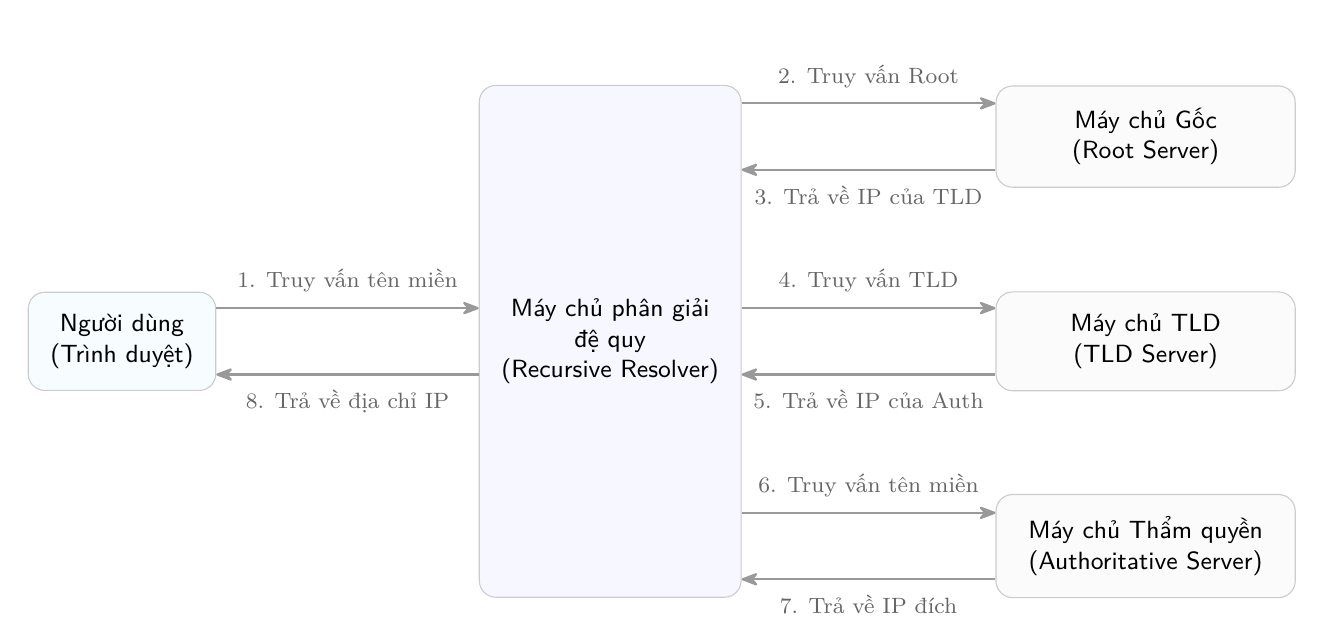
\begin{tikzpicture}[
    font=\sffamily\small,
    >={Stealth[round, scale=1.1]},
    client/.style={draw=gray!40, fill=cyan!3, rounded corners=6pt, inner sep=8pt, align=center, minimum height=1.2cm},
    resolver/.style={draw=gray!40, fill=blue!3, rounded corners=6pt, inner sep=8pt, align=center, minimum height=6.5cm, minimum width=2.8cm},
    server/.style={draw=gray!40, fill=gray!3, rounded corners=6pt, inner sep=8pt, align=center, minimum height=1.2cm, minimum width=3.8cm},
    arrow/.style={->, thick, gray!80, rounded corners=4pt},
    lbl/.style={text=gray!80!black, font=\footnotesize}
]

% Nodes
\node[client] (client) at (0, 0) {Người dùng\\(Trình duyệt)};
\node[resolver] (resolver) at (6.2, 0) {Máy chủ phân giải\\đệ quy\\(Recursive Resolver)};

\node[server] (root) at (13, 2.6) {Máy chủ Gốc\\(Root Server)};
\node[server] (tld) at (13, 0) {Máy chủ TLD\\(TLD Server)};
\node[server] (auth) at (13, -2.6) {Máy chủ Thẩm quyền\\(Authoritative Server)};

% Client <-> Resolver
\draw[arrow] ([yshift=12pt]client.east) -- ([yshift=12pt]resolver.west) node[midway, above=2pt, lbl] {1. Truy vấn tên miền};
\draw[arrow, <-] ([yshift=-12pt]client.east) -- ([yshift=-12pt]resolver.west) node[midway, below=2pt, lbl] {8. Trả về địa chỉ IP};

% Resolver <-> Root
\draw[arrow] ([yshift=12pt]resolver.east |- root.west) -- ([yshift=12pt]root.west) node[midway, above=2pt, lbl] {2. Truy vấn Root};
\draw[arrow, <-] ([yshift=-12pt]resolver.east |- root.west) -- ([yshift=-12pt]root.west) node[midway, below=2pt, lbl] {3. Trả về IP của TLD};

% Resolver <-> TLD
\draw[arrow] ([yshift=12pt]resolver.east |- tld.west) -- ([yshift=12pt]tld.west) node[midway, above=2pt, lbl] {4. Truy vấn TLD};
\draw[arrow, <-] ([yshift=-12pt]resolver.east |- tld.west) -- ([yshift=-12pt]tld.west) node[midway, below=2pt, lbl] {5. Trả về IP của Auth};

% Resolver <-> Auth
\draw[arrow] ([yshift=12pt]resolver.east |- auth.west) -- ([yshift=12pt]auth.west) node[midway, above=2pt, lbl] {6. Truy vấn tên miền};
\draw[arrow, <-] ([yshift=-12pt]resolver.east |- auth.west) -- ([yshift=-12pt]auth.west) node[midway, below=2pt, lbl] {7. Trả về IP đích};

\end{tikzpicture}

    \caption{Sơ đồ quy trình phân giải tên miền truyền thống}
    \label{fig:dns_traditional}
\end{figure}


\subsection{Cơ chế hố DNS (DNS Sinkhole)}
Hố DNS (DNS Sinkhole) là một kỹ thuật bảo mật hoạt động dựa trên nguyên lý chủ động cung cấp thông tin phân giải sai lệch đối với các tên miền được xác định là có rủi ro cao. Thay vì trả về địa chỉ IP thực tế của trang web lừa đảo, máy chủ DNS được cấu hình dưới dạng sinkhole sẽ trả về một địa chỉ IP không thể định tuyến (như \texttt{0.0.0.0}) hoặc địa chỉ IP của một máy chủ cảnh báo nội bộ (block page). Phương pháp này sở hữu ưu điểm vượt trội về hiệu năng do không cần trực tiếp phân tích nội dung gói tin của tầng ứng dụng. Kỹ thuật DNS sinkhole giúp quản trị viên vô hiệu hóa khả năng truy cập vào các chiến dịch tấn công giả mạo (phishing) trên quy mô lớn, đồng thời tối ưu hóa tài nguyên phần cứng để đáp ứng lưu lượng mạng cường độ cao.

\subsection{Các giao thức DNS bảo mật: DoH và DoT}
Giao thức DNS truyền thống hoạt động dựa trên UDP hoặc TCP qua cổng 53, truyền tải dữ liệu dưới dạng bản rõ (plaintext). Kiến trúc này tiềm ẩn rủi ro bị đánh chặn, theo dõi, hoặc giả mạo gói tin (DNS spoofing) thông qua các cuộc tấn công xen giữa (Man-in-the-Middle). Để khắc phục lỗ hổng này, các tiêu chuẩn mã hóa đường truyền DNS đã được ban hành và ứng dụng rộng rãi:
\begin{itemize}
    \item \textbf{DNS over TLS (DoT - RFC 7858):} Mã hóa trực tiếp các bản tin DNS thông qua giao thức TLS qua cổng 853 riêng biệt. DoT cung cấp mức độ bảo mật truyền tải cao, chống nghe lén hiệu quả ở tầng mạng nhưng có thể dễ dàng bị nhận diện và ngăn chặn bởi các hệ thống tường lửa dựa trên cổng giao tiếp.
    \item \textbf{DNS over HTTPS (DoH - RFC 8484):} Đóng gói các truy vấn DNS bên trong luồng dữ liệu HTTP/2 bảo mật qua cổng 443 thông dụng. Cơ chế này hòa trộn lưu lượng DNS vào lưu lượng duyệt web thông thường, gia tăng khả năng vượt qua các quy tắc lọc gói tin tĩnh và bảo vệ tối đa tính riêng tư của truy vấn.
\end{itemize}
Việc tích hợp các giao thức mã hóa này vào hệ thống phân giải tên miền không chỉ đảm bảo tính toàn vẹn của kết quả trả về mà còn che giấu mô hình truy vấn, gia tăng tính chủ động của hệ thống phòng thủ.

\section{Phân tích ngữ vựng và Trí tuệ nhân tạo}


\section{Công nghệ Backend}

Kiến trúc tầng xử lý dữ liệu (backend) của hệ thống đóng vai trò quyết định trong việc đáp ứng yêu cầu phân giải tên miền với độ trễ tối thiểu và độ tin cậy cao. Việc lựa chọn công nghệ được cân nhắc kỹ lưỡng dựa trên các tiêu chí về hiệu năng, khả năng xử lý đồng thời (concurrency) và tính tinh gọn khi đóng gói triển khai.

\subsection{Ngôn ngữ lập trình Go}
Ngôn ngữ Go (Golang) được sử dụng làm nền tảng cốt lõi để phát triển các module nội bộ, bao gồm máy chủ phân giải DNS (`dns-resolver`) và dịch vụ API trung tâm (`core-api`). Được thiết kế với cơ chế cấp phát bộ nhớ tối ưu và bộ dọn rác (garbage collector) hiệu quả, Go giảm thiểu đáng kể các rào cản về độ trễ thường gặp ở các ngôn ngữ thông dịch. Khả năng xử lý đồng thời thông qua mô hình goroutines và channels cho phép hệ thống tiếp nhận và phân tích hàng nghìn truy vấn DNS mỗi giây. Quá trình biên dịch tĩnh (statically typed) mã nguồn thành một tệp thực thi độc lập (single binary) giúp hệ thống loại bỏ các tệp phụ thuộc bên ngoài, tối ưu hóa quá trình đóng gói và vận hành qua Docker.

\subsection{Lưu trữ dữ liệu: SQLite và Redis}
Hệ thống áp dụng mô hình lưu trữ hỗn hợp nhằm khai thác ưu điểm của từng động cơ cơ sở dữ liệu đối với các loại dữ liệu đặc thù. 

SQLite được sử dụng để lưu trữ các thông tin mang tính bền vững như cấu hình hệ thống, bộ nhớ đệm WHOIS, danh sách miền tin cậy (whitelist), và các bản ghi đo lường hoạt động (telemetry). Dưới dạng một cơ sở dữ liệu nhúng (embedded database) không yêu cầu máy chủ nền tảng (serverless), SQLite loại bỏ hoàn toàn độ trễ giao tiếp mạng (network latency) giữa ứng dụng và cơ sở dữ liệu, đảm bảo tốc độ đọc ghi cục bộ đạt mức tối đa.

Bổ trợ cho SQLite là hệ thống Redis, được tích hợp nhằm vận hành bộ nhớ đệm tốc độ cao (in-memory cache) trên cơ sở bộ nhớ RAM. Redis đóng vai trò thiết yếu trong việc quản lý và tra cứu tập dữ liệu tình báo mối đe dọa (threat feed), nơi yêu cầu các thao tác kiểm tra phần tử (như lệnh \texttt{SISMEMBER}) phải được thực thi với độ phức tạp thời gian O(1). Cơ chế này đảm bảo mọi truy vấn tên miền đều được đối chiếu với cơ sở dữ liệu độc hại gần như tức thời trước khi kích hoạt quy trình phân tích ngữ vựng.

\subsection{Máy chủ proxy và bảo mật Caddy}
Caddy Server được triển khai dưới vai trò máy chủ proxy ngược (reverse proxy) để quản lý luồng giao tiếp mạng bên ngoài. Nhiệm vụ của phần mềm này là điều hướng lưu lượng truy cập HTTPS vào các điểm cuối (endpoints) tương ứng của hệ thống, bao gồm API và giao diện quản trị tĩnh (SPA). Lợi thế kỹ thuật cốt lõi của Caddy nằm ở khả năng tự động cấp phát, gia hạn và quản lý chứng chỉ bảo mật TLS thông qua giao thức ACME mà không đòi hỏi can thiệp thủ công. Việc ủy quyền lớp mã hóa truyền tải cho Caddy giúp phân tách rõ ràng trách nhiệm bảo mật mạng và logic nghiệp vụ, đồng thời giảm thiểu áp lực xử lý cho các module viết bằng Go ở phía sau.

\section{Công nghệ Frontend}

Giao diện quản trị (Operator UI) của dự án được thiết kế hướng tới mục tiêu trực quan hóa dữ liệu đo lường mạng (telemetry) và cung cấp khả năng cấu hình hệ thống tại thời gian thực. Để đáp ứng khối lượng thông tin lớn và đòi hỏi tốc độ phản hồi tức thì, kiến trúc phía máy khách (frontend) sử dụng bộ khung ứng dụng trang đơn (Single Page Application) kết hợp với các thư viện thành phần hiện đại.

\subsection{Kiến trúc Ứng dụng trang đơn (React SPA) và Tích hợp nhúng}
Giao diện người dùng được xây dựng trên nền tảng thư viện React dưới dạng Single Page Application (SPA). Cơ chế này cho phép trình duyệt tải toàn bộ mã định tuyến và cấu trúc giao diện ngay trong lần truy cập đầu tiên. Trong các phiên tương tác tiếp theo, dữ liệu được lấy và cập nhật bất đồng bộ thông qua các lệnh gọi API tới máy chủ trung tâm (`core-api`), loại bỏ tình trạng tải lại trang toàn phần (full page reload) và mang lại trải nghiệm điều hướng liền mạch. 

Điểm đặc thù trong quy trình triển khai của dự án là khối mã nguồn frontend sau khi được biên dịch (production build) sẽ được nhúng trực tiếp vào tệp thực thi của ngôn ngữ Go thông qua thư viện `embed`. Phương pháp tiếp cận này giúp loại bỏ nhu cầu thiết lập một máy chủ web độc lập (như Nginx hay Node.js) dành riêng cho frontend, đồng thời đồng bộ hóa hoàn toàn luồng phân phối phần mềm của cả hai phân hệ vào một khối duy nhất.

\subsection{Hệ thống thành phần giao diện với Tailwind CSS và Radix UI}
Để duy trì tính nhất quán thị giác và tối ưu phát triển, dự án áp dụng kiến trúc giao diện theo hướng Shadcn UI, kết hợp Tailwind CSS và các cấu trúc nguyên thủy từ Radix UI. Phương pháp này cung cấp các khối giao diện không định kiểu sẵn nhưng tuân thủ nghiêm ngặt tiêu chuẩn tiếp cận (accessibility) của W3C. Mô hình này cho phép tùy biến linh hoạt các phân hệ cốt lõi như danh sách ngoại lệ (Overrides), nhật ký rủi ro (Reports) và thông số kỹ thuật (System) mà không phụ thuộc vào các thư viện đóng gói nguyên khối. Sự kết hợp này giúp hệ thống tiêu chuẩn hóa hiển thị, duy trì độ phản hồi cao và giảm thiểu đáng kể mã nguồn CSS tĩnh phải duy trì thủ công.

\subsection{Trực quan hóa dữ liệu với Recharts}
Nhiệm vụ trọng tâm của giao diện quản trị là biểu diễn đồ họa các xu hướng phân giải tên miền và phân bố điểm số rủi ro. Yêu cầu này được giải quyết thông qua thư viện Recharts, một giải pháp kết xuất biểu đồ thiết kế riêng cho hệ sinh thái React. Recharts được ứng dụng để khởi tạo các biểu đồ đường (line charts) nhằm theo dõi lưu lượng truy vấn theo thời gian và các biểu đồ phân bổ (breakdown charts) phân loại tỷ trọng rủi ro theo ba ngưỡng: an toàn (SAFE), đáng ngờ (SUSPICIOUS) và độc hại (MALICIOUS). Việc chuyển hóa các tham số phân tích thành biểu đồ động giúp quản trị viên hệ thống nhanh chóng nhận dạng các mẫu hình lưu lượng bất thường (anomalies) hoặc các chiến dịch phát tán mã độc quy mô lớn.

\chapter{PHÂN TÍCH VÀ THIẾT KẾ HỆ THỐNG}
\section{Phân tích yêu cầu}


\section{Kiến trúc tổng thể}


\section{Thiết kế luồng phân tích rủi ro}

Luồng phân tích rủi ro của hệ thống Safe Zone được thiết kế dựa trên triết lý kiểm tra đa lớp (multi-layered pipeline), nhằm cân bằng giữa tốc độ phân giải DNS siêu tốc và độ chính xác trong việc phát hiện tên miền lừa đảo. Mỗi truy vấn khi đi vào hệ thống sẽ lần lượt đi qua các bộ lọc từ đơn giản đến phức tạp, giúp tối ưu hóa tài nguyên tính toán và giảm thiểu độ trễ cho người dùng cuối.

\begin{figure}[H]
    \centering
    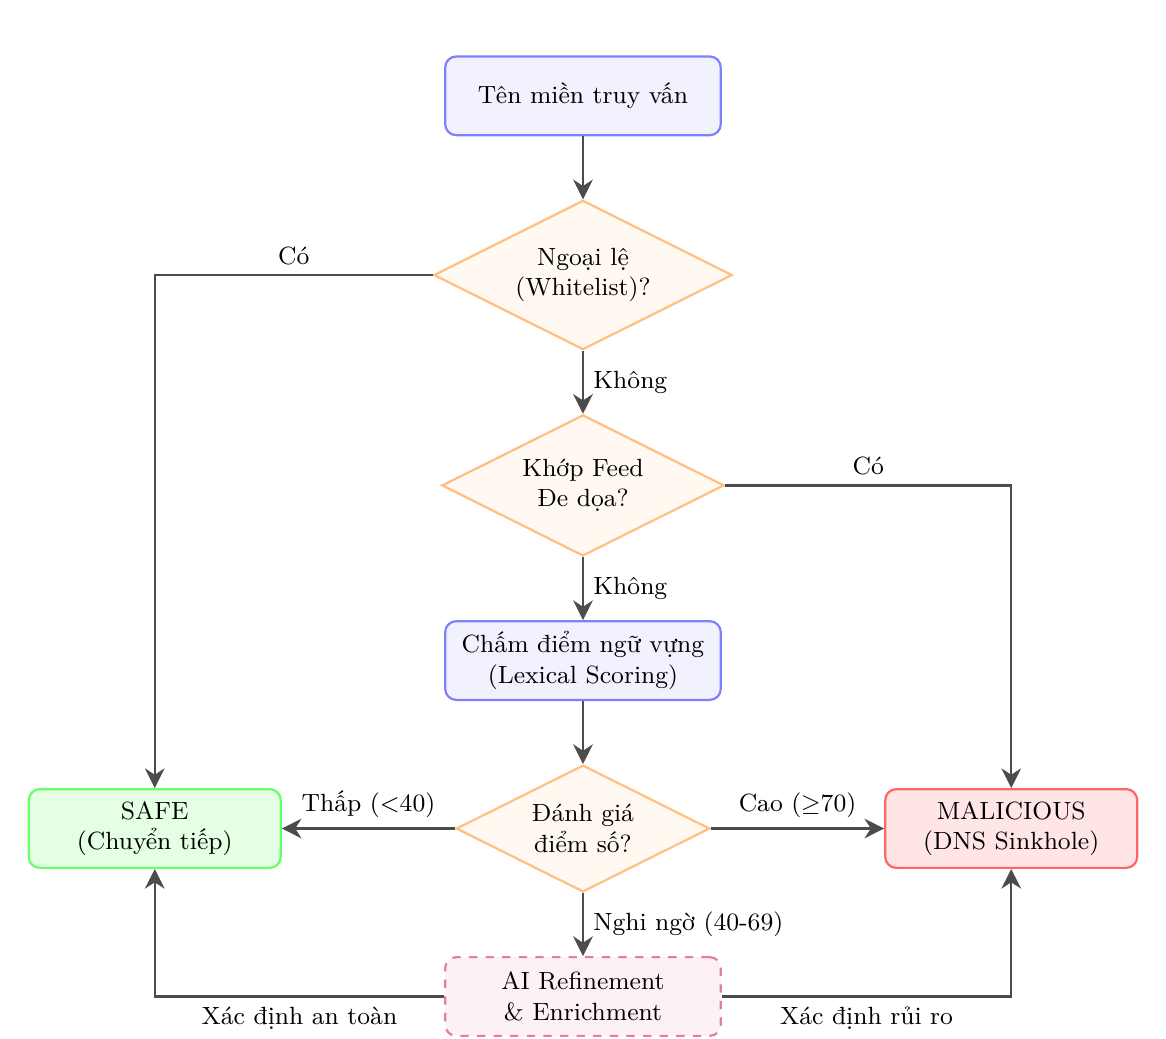
\begin{tikzpicture}[
        node distance=1cm and 3cm,
        process/.style={rectangle, draw=blue!50, thick, rounded corners, fill=blue!5, minimum width=3.5cm, minimum height=1cm, align=center},
        decision/.style={diamond, draw=orange!50, thick, fill=orange!5, minimum width=3.2cm, minimum height=1.2cm, align=center, aspect=2},
        safe/.style={rectangle, draw=green!60, thick, rounded corners, fill=green!10, minimum width=3.2cm, minimum height=1cm, align=center},
        malicious/.style={rectangle, draw=red!60, thick, rounded corners, fill=red!10, minimum width=3.2cm, minimum height=1cm, align=center},
        ai/.style={rectangle, draw=purple!50, thick, rounded corners, fill=purple!5, dashed, minimum width=3.5cm, minimum height=1cm, align=center},
        arrow/.style={-{Stealth[length=2.5mm, width=2.5mm]}, thick, draw=black!70},
        font=\small
    ]

    % Central Column
    \node (input) [process] {Tên miền truy vấn};
    \node (whitelist) [decision, below=0.8cm of input] {Ngoại lệ\\(Whitelist)?};
    \node (threat_feed) [decision, below=0.8cm of whitelist] {Khớp Feed\\Đe dọa?};
    \node (lexical) [process, below=0.8cm of threat_feed] {Chấm điểm ngữ vựng\\(Lexical Scoring)};
    \node (score_check) [decision, below=0.8cm of lexical] {Đánh giá\\điểm số?};
    \node (ai_refinement) [ai, below=0.8cm of score_check] {AI Refinement\\\& Enrichment};

    % Left & Right Columns
    % Place safe_verdict aligned horizontally with score_check
    \node (safe_verdict) [safe, left=2.2cm of score_check] {SAFE\\(Chuyển tiếp)};
    \node (malicious_verdict) [malicious, right=2.2cm of score_check] {MALICIOUS\\(DNS Sinkhole)};

    % Arrows - Vertical
    \draw [arrow] (input) -- (whitelist);
    \draw [arrow] (whitelist) -- (threat_feed) node[midway, right] {Không};
    \draw [arrow] (threat_feed) -- (lexical) node[midway, right] {Không};
    \draw [arrow] (lexical) -- (score_check);
    \draw [arrow] (score_check) -- (ai_refinement) node[midway, right] {Nghi ngờ (40-69)};

    % Lateral Arrows
    \draw [arrow] (whitelist) -| (safe_verdict) node[pos=0.25, above] {Có};
    \draw [arrow] (threat_feed) -| (malicious_verdict) node[pos=0.25, above] {Có};
    \draw [arrow] (score_check) -- (safe_verdict) node[midway, above] {Thấp (<40)};
    \draw [arrow] (score_check) -- (malicious_verdict) node[midway, above] {Cao ($\ge$70)};
    \draw [arrow] (ai_refinement) -| (safe_verdict) node[pos=0.25, below] {Xác định an toàn};
    \draw [arrow] (ai_refinement) -| (malicious_verdict) node[pos=0.25, below] {Xác định rủi ro};

    \end{tikzpicture}
    \caption{Sơ đồ luồng phân tích rủi ro tên miền (Risk Analysis Pipeline)}
    \label{fig:risk_analysis_flow}
\end{figure}


Quá trình phân tích rủi ro được chia thành các giai đoạn tuần tự sau:

\textbf{1. Kiểm tra danh sách ngoại lệ (Whitelist):}
Bước đầu tiên trong luồng xử lý là đối chiếu tên miền với danh sách ngoại lệ. Hệ thống triển khai thuật toán cấu trúc dữ liệu xác suất (Bloom filter) được nạp trực tiếp vào bộ nhớ chính (RAM) để đảm bảo thời gian tra cứu gần như tức thời ($O(1)$). Nếu tên miền khớp với danh sách ngoại lệ, hệ thống bỏ qua toàn bộ các bước phân tích phía sau và đánh giá tên miền là an toàn (SAFE), sau đó chuyển tiếp truy vấn đến DNS thượng nguồn. Cơ chế này giúp loại bỏ các cảnh báo nhầm (false positives) đối với các dịch vụ hợp lệ phổ biến.

\textbf{2. Đối chiếu tình báo mối đe dọa (Threat Feed):}
Trường hợp tên miền không nằm trong danh sách ngoại lệ, hệ thống tiến hành kiểm tra trên tập dữ liệu tình báo mối đe dọa. Dữ liệu này được đồng bộ định kỳ vào cấu trúc Set của Redis, cho phép tra cứu khớp hoàn toàn (exact match) hoặc khớp hậu tố phụ (suffix match). Bất kỳ sự trùng khớp nào tại bước này đều mang tính xác định luận (deterministic), dẫn đến việc tên miền bị phán định là độc hại (MALICIOUS) ngay lập tức và hệ thống thực hiện hố DNS (DNS sinkhole).

\textbf{3. Chấm điểm ngữ vựng (Lexical Scoring):}
Lớp bảo vệ thứ ba đóng vai trò cốt lõi trong việc phát hiện các hình thái lừa đảo mới (zero-day phishing) chưa từng xuất hiện trong danh sách chặn. Luồng phân tích ngữ vựng áp dụng các quy tắc khám phá (heuristic) dựa trên tám tín hiệu cụ thể. Tiêu biểu là việc tính toán mức độ hỗn loạn của chuỗi ký tự (Shannon Entropy) để nhận diện thuật toán sinh tên miền tự động (DGA), hoặc phân tích khoảng cách chỉnh sửa để chống giả mạo thương hiệu (brand spoofing). Kết quả của quá trình này là một điểm số rủi ro dao động từ 0 đến 100. Dựa vào điểm số, hệ thống có ba hướng rẽ nhánh:
\begin{itemize}
    \item \textbf{Thấp} ($< 40$): Tên miền được xem là an toàn (SAFE).
    \item \textbf{Cao} ($\ge 70$): Tên miền bị đánh giá là độc hại (MALICIOUS).
    \item \textbf{Nghi ngờ} ($40 - 69$): Tên miền được chuyển sang giai đoạn phân tích tăng cường.
\end{itemize}

\textbf{4. Phân tích tăng cường (AI Refinement):}
Đối với các tên miền có ranh giới rủi ro mờ nhạt, hệ thống có thể kích hoạt tùy chọn phân tích bổ sung thông qua mô hình học ngôn ngữ lớn (ví dụ: Gemini 2.5 Flash Lite). Bước này tự động thu thập thêm thông tin cấu trúc (WHOIS) từ bộ đệm SQLite và phân tích chứng chỉ TLS nhằm cung cấp ngữ cảnh (context) mở rộng cho AI phán định. 

Điều làm nên tính bền bỉ của hệ thống tại lớp này là kiến trúc mở khi lỗi (fail-open). Nếu liên kết với API của mô hình AI bị gián đoạn hoặc thời gian chờ vượt quá giới hạn (timeout), hệ thống sẽ chủ động hạ cấp đánh giá rủi ro để tên miền được đi qua. Cơ chế này đảm bảo sự cố tại một tiến trình phụ trợ không làm nghẽn toàn bộ luồng phân giải DNS, giúp duy trì kết nối mạng của thiết bị ở mức tối đa.

\section{Thiết kế cơ sở dữ liệu và cache}


\chapter{TRIỂN KHAI CHI TIẾT}
\section{Cấu trúc mã nguồn}


\section{Triển khai hệ thống DNS}

Phân hệ \texttt{dns-resolver} đóng vai trò là cửa ngõ giao tiếp trực tiếp với thiết bị của người dùng. Tuy nhiên, để đảm bảo an ninh, tính khả dụng và khả năng mở rộng, hệ thống DNS không đứng độc lập mà được triển khai phối hợp cùng các dịch vụ lõi khác trong một kiến trúc mạng nội bộ bảo mật (Docker Internal Network).

\begin{figure}[H]
    \centering
    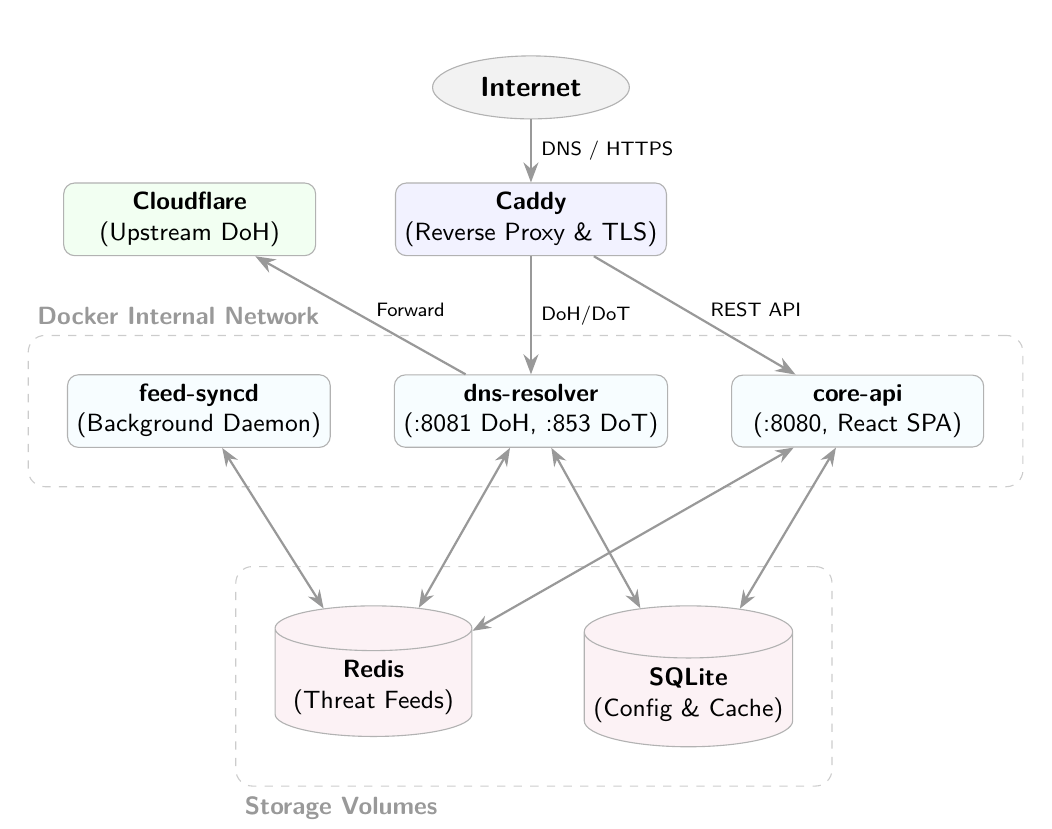
\begin{tikzpicture}[
        node distance=1.2cm and 1cm,
        box/.style={rectangle, draw=gray!60, rounded corners=4pt, minimum width=3.2cm, minimum height=0.9cm, align=center, fill=cyan!3, font=\sffamily\small},
        db/.style={cylinder, draw=gray!60, shape border rotate=90, aspect=0.25, minimum width=2.5cm, minimum height=1.2cm, align=center, fill=purple!5, font=\sffamily\small},
        group/.style={rectangle, draw=gray!40, rounded corners=6pt, inner sep=14pt, dashed},
        arrow/.style={-{Stealth[scale=1.1]}, thick, draw=gray!80},
        biarrow/.style={<->, >=Stealth, thick, draw=gray!80}
    ]
        % Internet & Proxy
        \node[ellipse, draw=gray!60, fill=gray!10, minimum width=2.5cm, minimum height=0.8cm, font=\sffamily\bfseries] (internet) {Internet};
        \node[box, below=0.8cm of internet, fill=blue!5] (caddy) {\textbf{Caddy}\\(Reverse Proxy \& TLS)};
        
        \draw[arrow] (internet) -- (caddy) node[midway, right, font=\sffamily\scriptsize] {DNS / HTTPS};

        % Upstream (Left of Caddy)
        \node[box, left=1cm of caddy, fill=green!5] (upstream) {\textbf{Cloudflare}\\(Upstream DoH)};

        % Core Services
        \node[box, below=1.5cm of caddy] (dns) {\textbf{dns-resolver}\\(:8081 DoH, :853 DoT)};
        \node[box, right=0.8cm of dns] (api) {\textbf{core-api}\\(:8080, React SPA)};
        \node[box, left=0.8cm of dns] (feed) {\textbf{feed-syncd}\\(Background Daemon)};

        % Group Docker
        \node[group, fit=(dns)(api)(feed)] (docker_group) {};
        \node[above right, font=\sffamily\bfseries\small, text=gray!80] at (docker_group.north west) {Docker Internal Network};

        % Connections from Caddy
        \draw[arrow] (caddy) -- (dns) node[midway, right, font=\sffamily\scriptsize] {DoH/DoT};
        \draw[arrow] (caddy) -- (api) node[midway, right, xshift=2pt, yshift=2pt, font=\sffamily\scriptsize] {REST API};

        % Connection to Upstream
        \draw[arrow] (dns) -- (upstream) node[midway, right, xshift=2pt, yshift=2pt, font=\sffamily\scriptsize] {Forward};

        % Databases
        \node[db, below=2cm of dns, xshift=-2cm] (redis) {\textbf{Redis}\\(Threat Feeds)};
        \node[db, below=2cm of dns, xshift=2cm] (sqlite) {\textbf{SQLite}\\(Config \& Cache)};

        % Group Storage
        \node[group, fit=(redis)(sqlite)] (storage_group) {};
        \node[below right, font=\sffamily\bfseries\small, text=gray!80] at (storage_group.south west) {Storage Volumes};

        % DB Connections
        \draw[biarrow] (feed) -- (redis);
        \draw[biarrow] (dns) -- (redis);
        \draw[biarrow] (dns) -- (sqlite);
        \draw[biarrow] (api) -- (sqlite);
        \draw[biarrow] (api) -- (redis);

    \end{tikzpicture}
    \caption{Kiến trúc triển khai mạng và dịch vụ (Deployment Architecture) của Safe Zone}
    \label{fig:deployment_architecture}
\end{figure}

Quá trình triển khai thực tế của hệ thống phân giải tên miền được thiết kế theo nguyên tắc thu hẹp bề mặt tấn công (attack surface reduction) và tối ưu hóa luồng giao tiếp nội bộ.

\textbf{Điểm vào duy nhất với Reverse Proxy}

Thay vì mở trực tiếp các cổng dịch vụ ra ngoài Internet, hệ thống sử dụng Caddy làm máy chủ ủy quyền ngược (reverse proxy). Caddy chịu trách nhiệm quản lý tự động chứng chỉ SSL/TLS, tiếp nhận mọi lưu lượng HTTP/HTTPS và phân luồng (routing) dựa trên tên miền con hoặc đường dẫn. Các truy vấn DNS over HTTPS (DoH) sẽ được định tuyến an toàn đến \texttt{dns-resolver} qua cổng nội bộ \texttt{8081}, trong khi các truy vấn quản trị được chuyển hướng đến \texttt{core-api} tại cổng \texttt{8080}. Thiết kế này đảm bảo toàn bộ giao tiếp giữa các tiến trình Go diễn ra hoàn toàn trong không gian mạng ảo của Docker (Docker Internal Network) mà không bị phơi nhiễm ra môi trường ngoài.

\textbf{Giao tiếp với không gian lưu trữ}

Các bộ nhớ dữ liệu bao gồm Redis (chứa tập hợp tình báo mối đe dọa lớn) và SQLite (chứa siêu dữ liệu cấu hình, bộ nhớ đệm WHOIS) được cách ly trong khối Storage Volumes. Tiến trình \texttt{dns-resolver} duy trì kết nối liên tục (persistent connection) tốc độ cao với Redis để kiểm tra trạng thái tên miền độc hại trong thời gian tính bằng micro-giây. Song song đó, tiến trình \texttt{feed-syncd} chạy ngầm định kỳ kéo dữ liệu mới từ các nguồn cấp (feeds) và cập nhật trực tiếp vào Redis thông qua các lệnh nguyên tử (atomic operations) nhằm đảm bảo \texttt{dns-resolver} luôn có dữ liệu mới nhất mà không gây khóa luồng (thread blocking).

\textbf{Kiến trúc phân giải ngược dòng (Upstream Forwarding)}

Đối với các tên miền an toàn, \texttt{dns-resolver} không tự thực hiện phân giải đệ quy toàn trình (full recursive lookup) để tối ưu độ trễ. Thay vào đó, hệ thống đóng vai trò như một bộ chuyển tiếp (forwarder) đến các máy chủ DNS ngược dòng (upstream) tốc độ cao và đề cao quyền riêng tư như Cloudflare thông qua đường hầm mã hóa DoH. Việc này vừa tận dụng được hệ thống bộ nhớ đệm khổng lồ của Upstream, vừa che giấu được thói quen duyệt web của người dùng đầu cuối khỏi các nhà cung cấp dịch vụ mạng (ISP).

\section{Triển khai dịch vụ phân tích và cập nhật nguồn dữ liệu}


\section{Triển khai giao diện quản trị}

Giao diện quản trị của hệ thống Safe Zone được triển khai dưới dạng Ứng dụng Trang Đơn (Single Page Application - SPA) nhằm cung cấp trải nghiệm mượt mà, hạn chế tối đa độ trễ phản hồi khi tương tác với khối lượng dữ liệu giám sát lớn. 

Kiến trúc triển khai mặt trước (Frontend) tuân thủ mô hình tách biệt hoàn toàn giữa Tầng Hiển thị (View Layer) và Tầng Quản lý Trạng thái (State Management):

\begin{figure}[H]
    \centering
    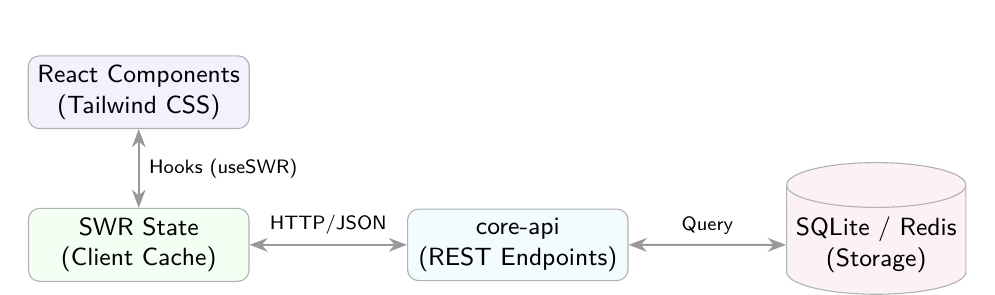
\begin{tikzpicture}[
        node distance=2.2cm,
        box/.style={rectangle, draw=gray!60, rounded corners=4pt, minimum width=2.8cm, minimum height=0.8cm, align=center, fill=blue!5, font=\sffamily\small},
        db/.style={cylinder, draw=gray!60, shape border rotate=90, aspect=0.25, minimum width=2cm, minimum height=1.2cm, align=center, fill=purple!5, font=\sffamily\small},
        biarrow/.style={<->, >=Stealth, thick, draw=gray!80}
    ]
        % Nodes
        \node[box] (ui) {React Components\\(Tailwind CSS)};
        \node[box, below=1cm of ui, fill=green!5] (swr) {SWR State\\(Client Cache)};
        \node[box, right=2cm of swr, fill=cyan!5] (api) {core-api\\(REST Endpoints)};
        \node[db, right=2cm of api] (db) {SQLite / Redis\\(Storage)};

        % Connections
        \draw[biarrow] (ui) -- (swr) node[midway, right, font=\sffamily\scriptsize] {Hooks (useSWR)};
        \draw[biarrow] (swr) -- (api) node[midway, above, font=\sffamily\scriptsize] {HTTP/JSON};
        \draw[biarrow] (api) -- (db) node[midway, above, font=\sffamily\scriptsize] {Query};
    \end{tikzpicture}
    \caption{Luồng dữ liệu và quản lý trạng thái của Giao diện Quản trị}
    \label{fig:ui_data_flow}
\end{figure}

Các kỹ thuật triển khai cốt lõi bao gồm:
\begin{itemize}
    \item \textbf{Đồng bộ trạng thái từ xa (Remote State Cache):} Hệ thống sử dụng thư viện \texttt{SWR} để quản lý trạng thái dữ liệu lấy từ API. Dữ liệu cấu hình, danh sách chặn lọc và số liệu giám sát được lưu trữ an toàn trong bộ nhớ đệm của trình duyệt. Giao diện luôn được hiển thị lập tức từ bộ đệm, song song với việc gọi API ngầm để xác thực lại tính mới của dữ liệu (Stale-while-revalidate), đảm bảo quản trị viên không bị gián đoạn bởi các màn hình chờ tải (Loading Spinners).
    \item \textbf{Trực quan hóa dữ liệu theo thời gian thực:} Tích hợp động cơ vẽ biểu đồ \texttt{Recharts} để thống kê lưu lượng DNS (Telemetry). Dữ liệu được tổng hợp (aggregate) và phân trang trực tiếp từ bộ đệm của \texttt{core-api}, giúp biểu đồ duy trì tốc độ khung hình (FPS) ổn định ngay cả khi hiển thị phân tích của hàng ngàn sự kiện truy vấn cùng lúc.
    \item \textbf{Tối ưu hóa tác vụ mạng (Network Optimization):} Xây dựng hệ thống form tương tác (ví dụ: công cụ cấu hình danh sách đen/trắng, công cụ phân tích rủi ro tên miền độc lập) được bọc trong các Hook bất đồng bộ, tự động xử lý thử lại khi lỗi mạng (network retry) và triệt tiêu các lệnh gọi trùng lặp (debounce) để giảm thiểu áp lực tải cho Backend.
\end{itemize}

Kết quả thực tế sau khi triển khai hệ thống giao diện:

\begin{figure}[H]
    \centering
    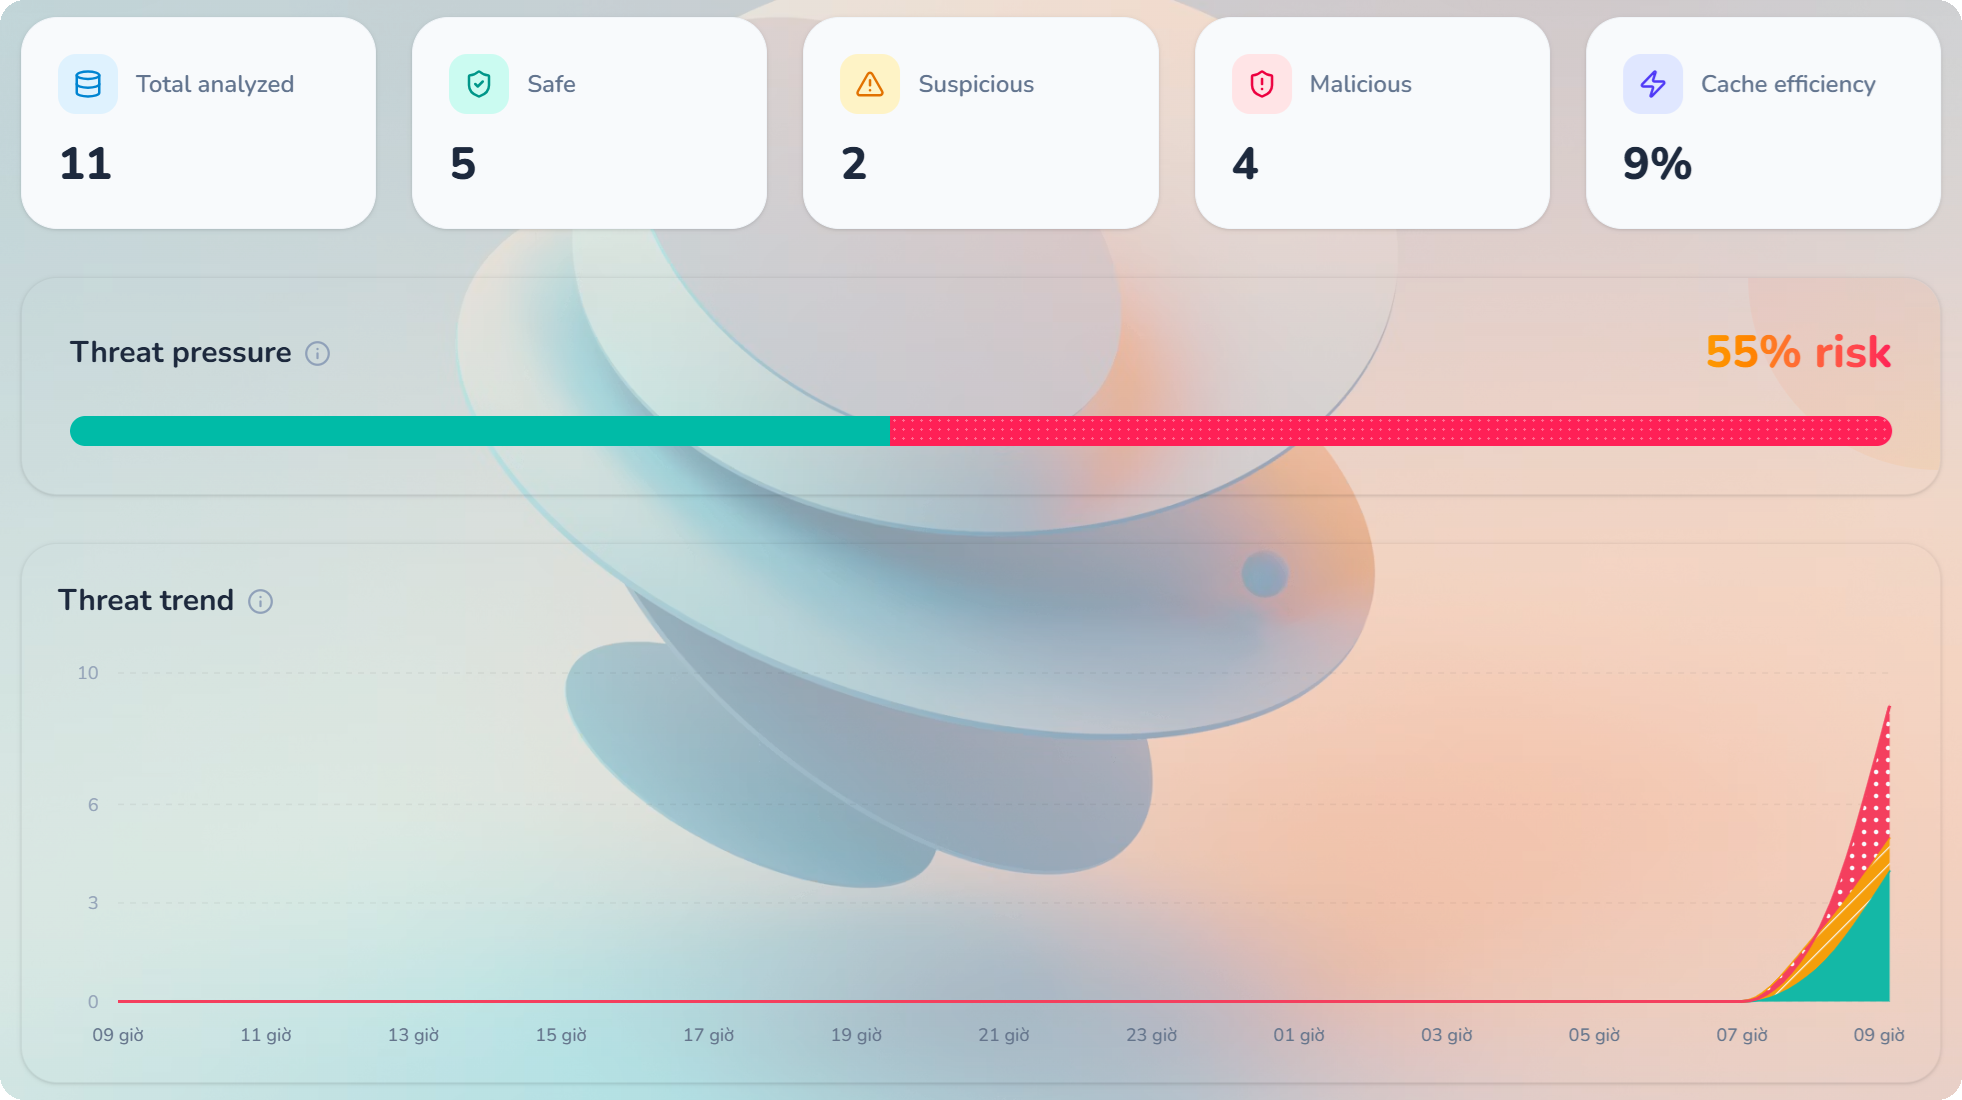
\includegraphics[width=0.9\textwidth]{img/ui_telemetry_1.png} \\
    \vspace{0.5cm}
    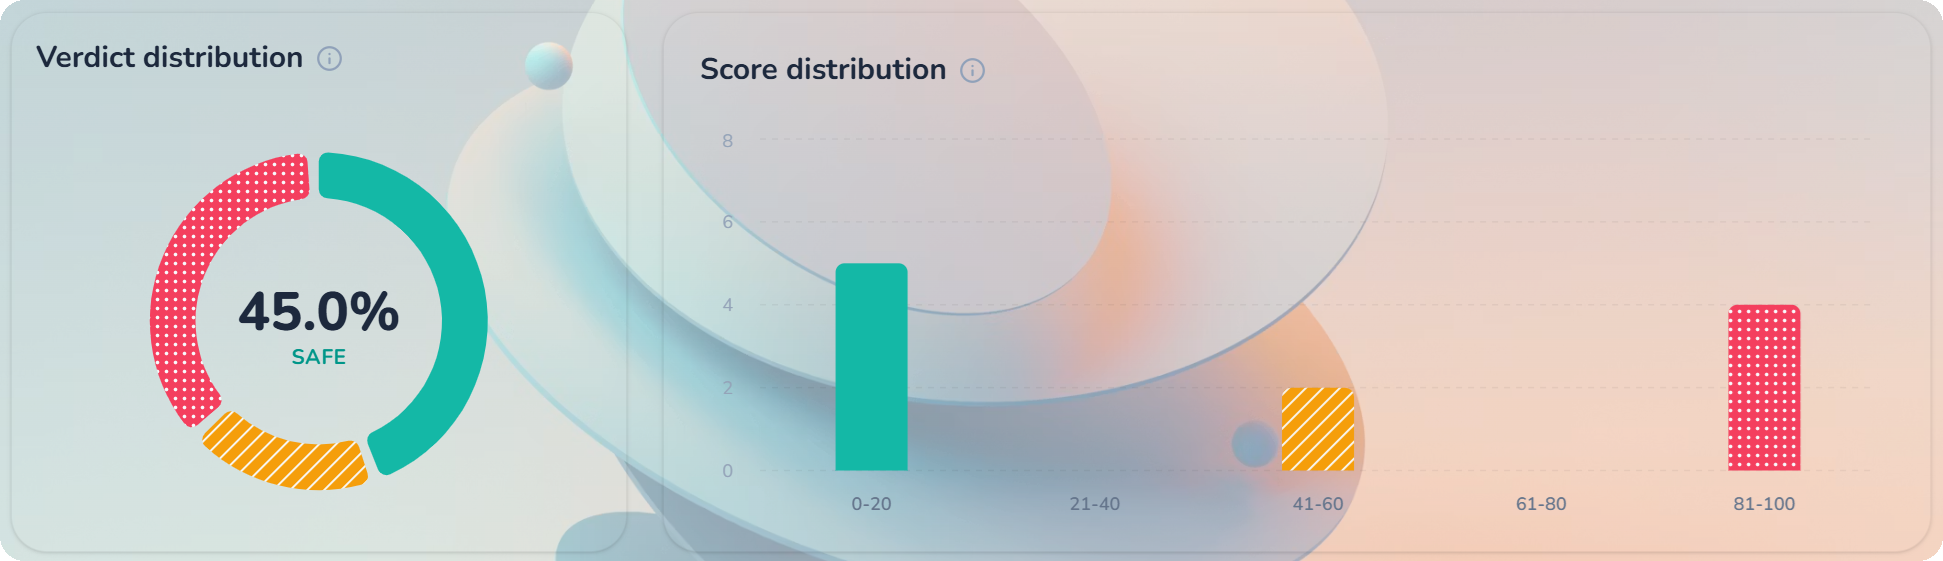
\includegraphics[width=0.9\textwidth]{img/ui_telemetry_2.png}
    \caption{Giao diện Bảng điều khiển (Telemetry) hiển thị thống kê truy vấn và phân phối rủi ro}
    \label{fig:ui_telemetry}
\end{figure}

Bảng điều khiển (Telemetry) đóng vai trò giám sát trung tâm (Hình \ref{fig:ui_telemetry}). Các biểu đồ động trực quan hóa tần suất truy vấn, tỷ lệ phân giải thành công và hiệu suất bộ nhớ đệm giúp quản trị viên đánh giá nhanh mức độ đe dọa (Threat Pressure) trong hệ thống mạng.

\begin{figure}[H]
    \centering
    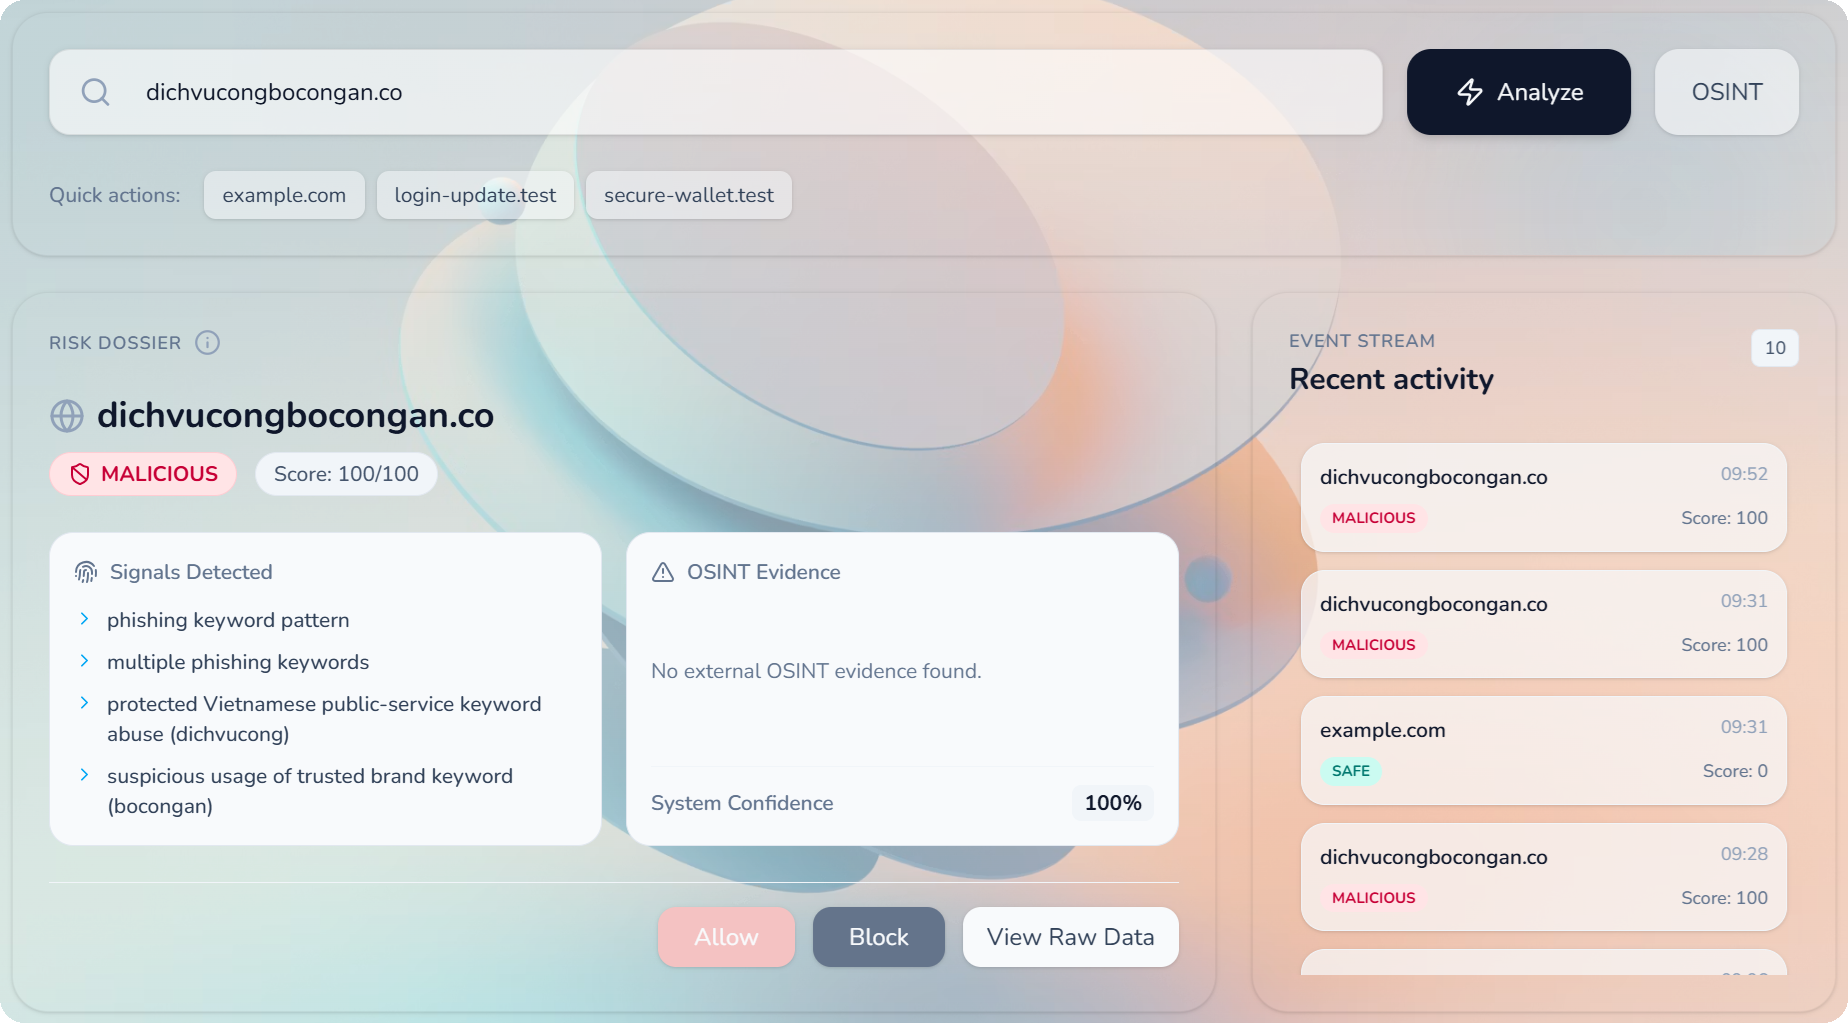
\includegraphics[width=0.9\textwidth]{img/ui_analysis_1.png} \\
    \vspace{0.5cm}
    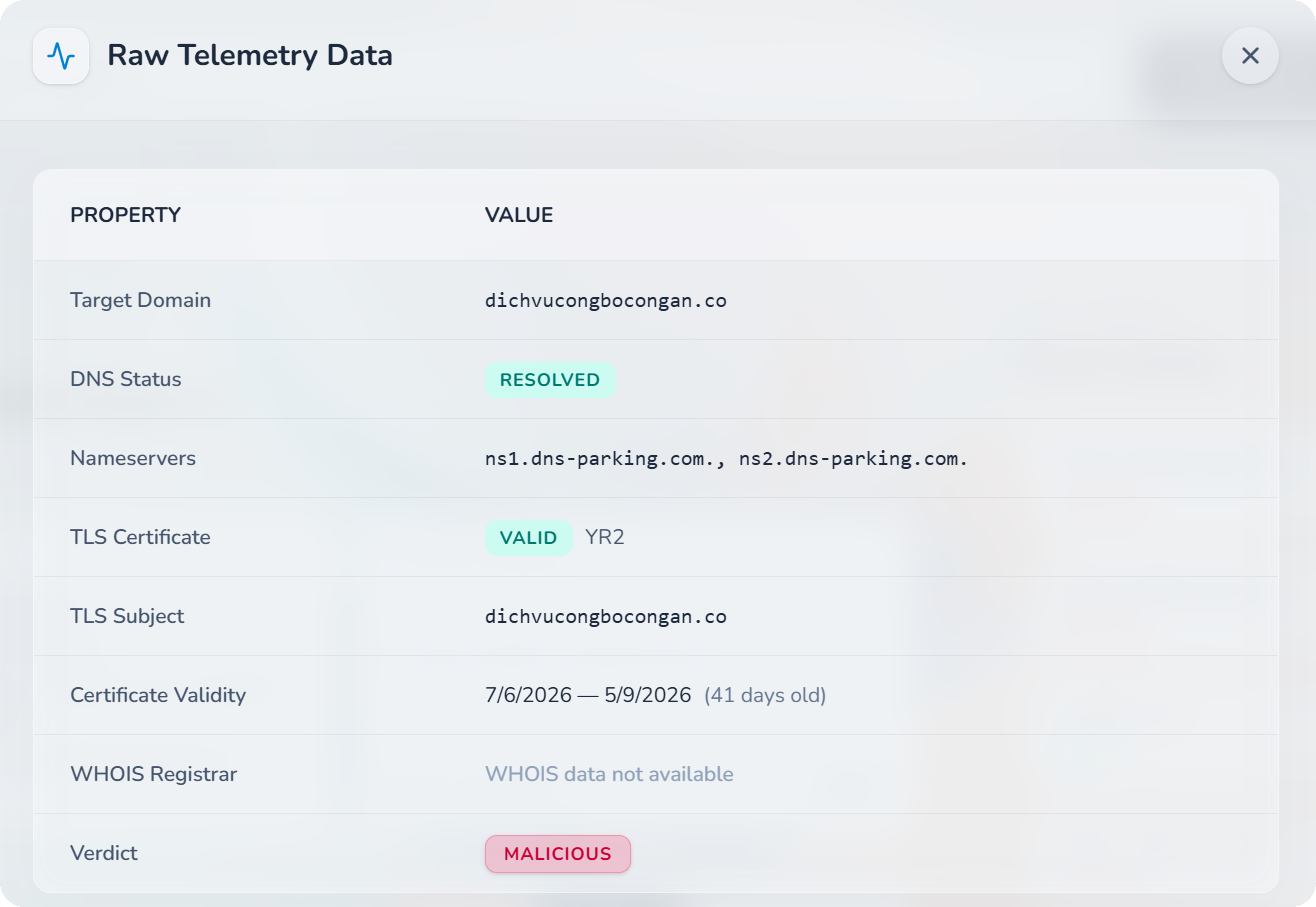
\includegraphics[width=0.9\textwidth]{img/ui_analysis_2.png}
    \caption{Giao diện Phân tích rủi ro tên miền động (Domain Analysis)}
    \label{fig:ui_analysis}
\end{figure}

Giao diện Phân tích (Domain Analysis) cung cấp khả năng kiểm tra sâu một tên miền bất kỳ (Hình \ref{fig:ui_analysis}). Việc bóc tách chi tiết các đặc trưng ngữ vựng (Lexical Features) kết hợp với kết quả suy luận AI mang lại tính minh bạch, giúp người quản trị dễ dàng xác minh tính chính xác của hệ thống.

\begin{figure}[H]
    \centering
    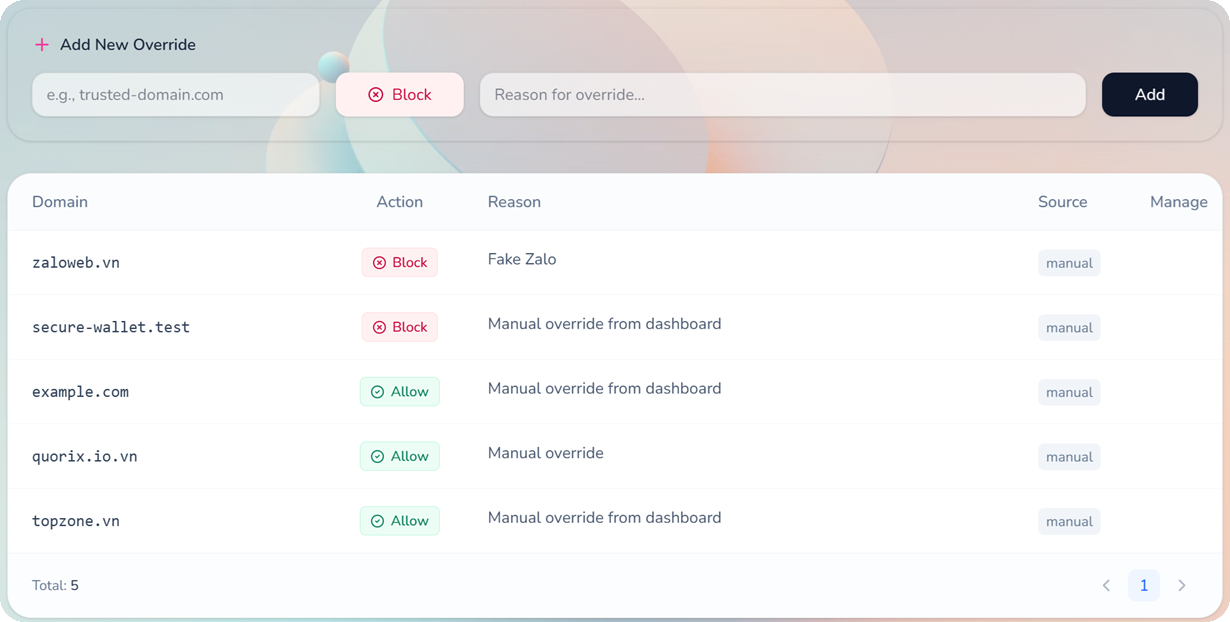
\includegraphics[width=0.9\textwidth]{img/ui_overrides.png} 
    \caption{Giao diện Quản lý danh sách cấu hình ngoại lệ (Overrides)}
    \label{fig:ui_overrides}
\end{figure}

Giao diện Quản lý ngoại lệ (Overrides) là thiết yếu để kiểm soát luồng phân giải (Hình \ref{fig:ui_overrides}). Việc lập Danh sách trắng (Whitelist) và Danh sách đen (Blacklist) giúp giảm cảnh báo nhầm (False Positive) và chủ động chặn đứng tức thời các mối đe dọa tại tầng DNS Resolver.

\chapter{ĐÁNH GIÁ BẢO MẬT, KIỂM THỬ VÀ VẬN HÀNH}
\section{Đánh giá hiệu năng và độ trễ}
Hiệu năng và độ trễ là tiêu chí trọng tâm của hệ thống phân giải tên miền (DNS Resolver), nhất là khi kết hợp chấm điểm ngữ vựng và đối chiếu tình báo mối đe dọa. Việc đánh giá Safe Zone được thực hiện bằng công cụ giả lập tải trong môi trường độc lập để đảm bảo khách quan.

\subsection{Đánh giá độ trễ phân giải (Latency)}

Thử nghiệm đo lường thời gian đáp ứng của hệ thống qua 3 kịch bản: truy vấn từ bộ nhớ đệm RAM (Redis Cache Hit), từ cơ sở dữ liệu cục bộ (SQLite Local Hit), và truy vấn mới cần phân tích ngữ vựng cục bộ (Cache Miss).

\begin{figure}[H]
    \centering
    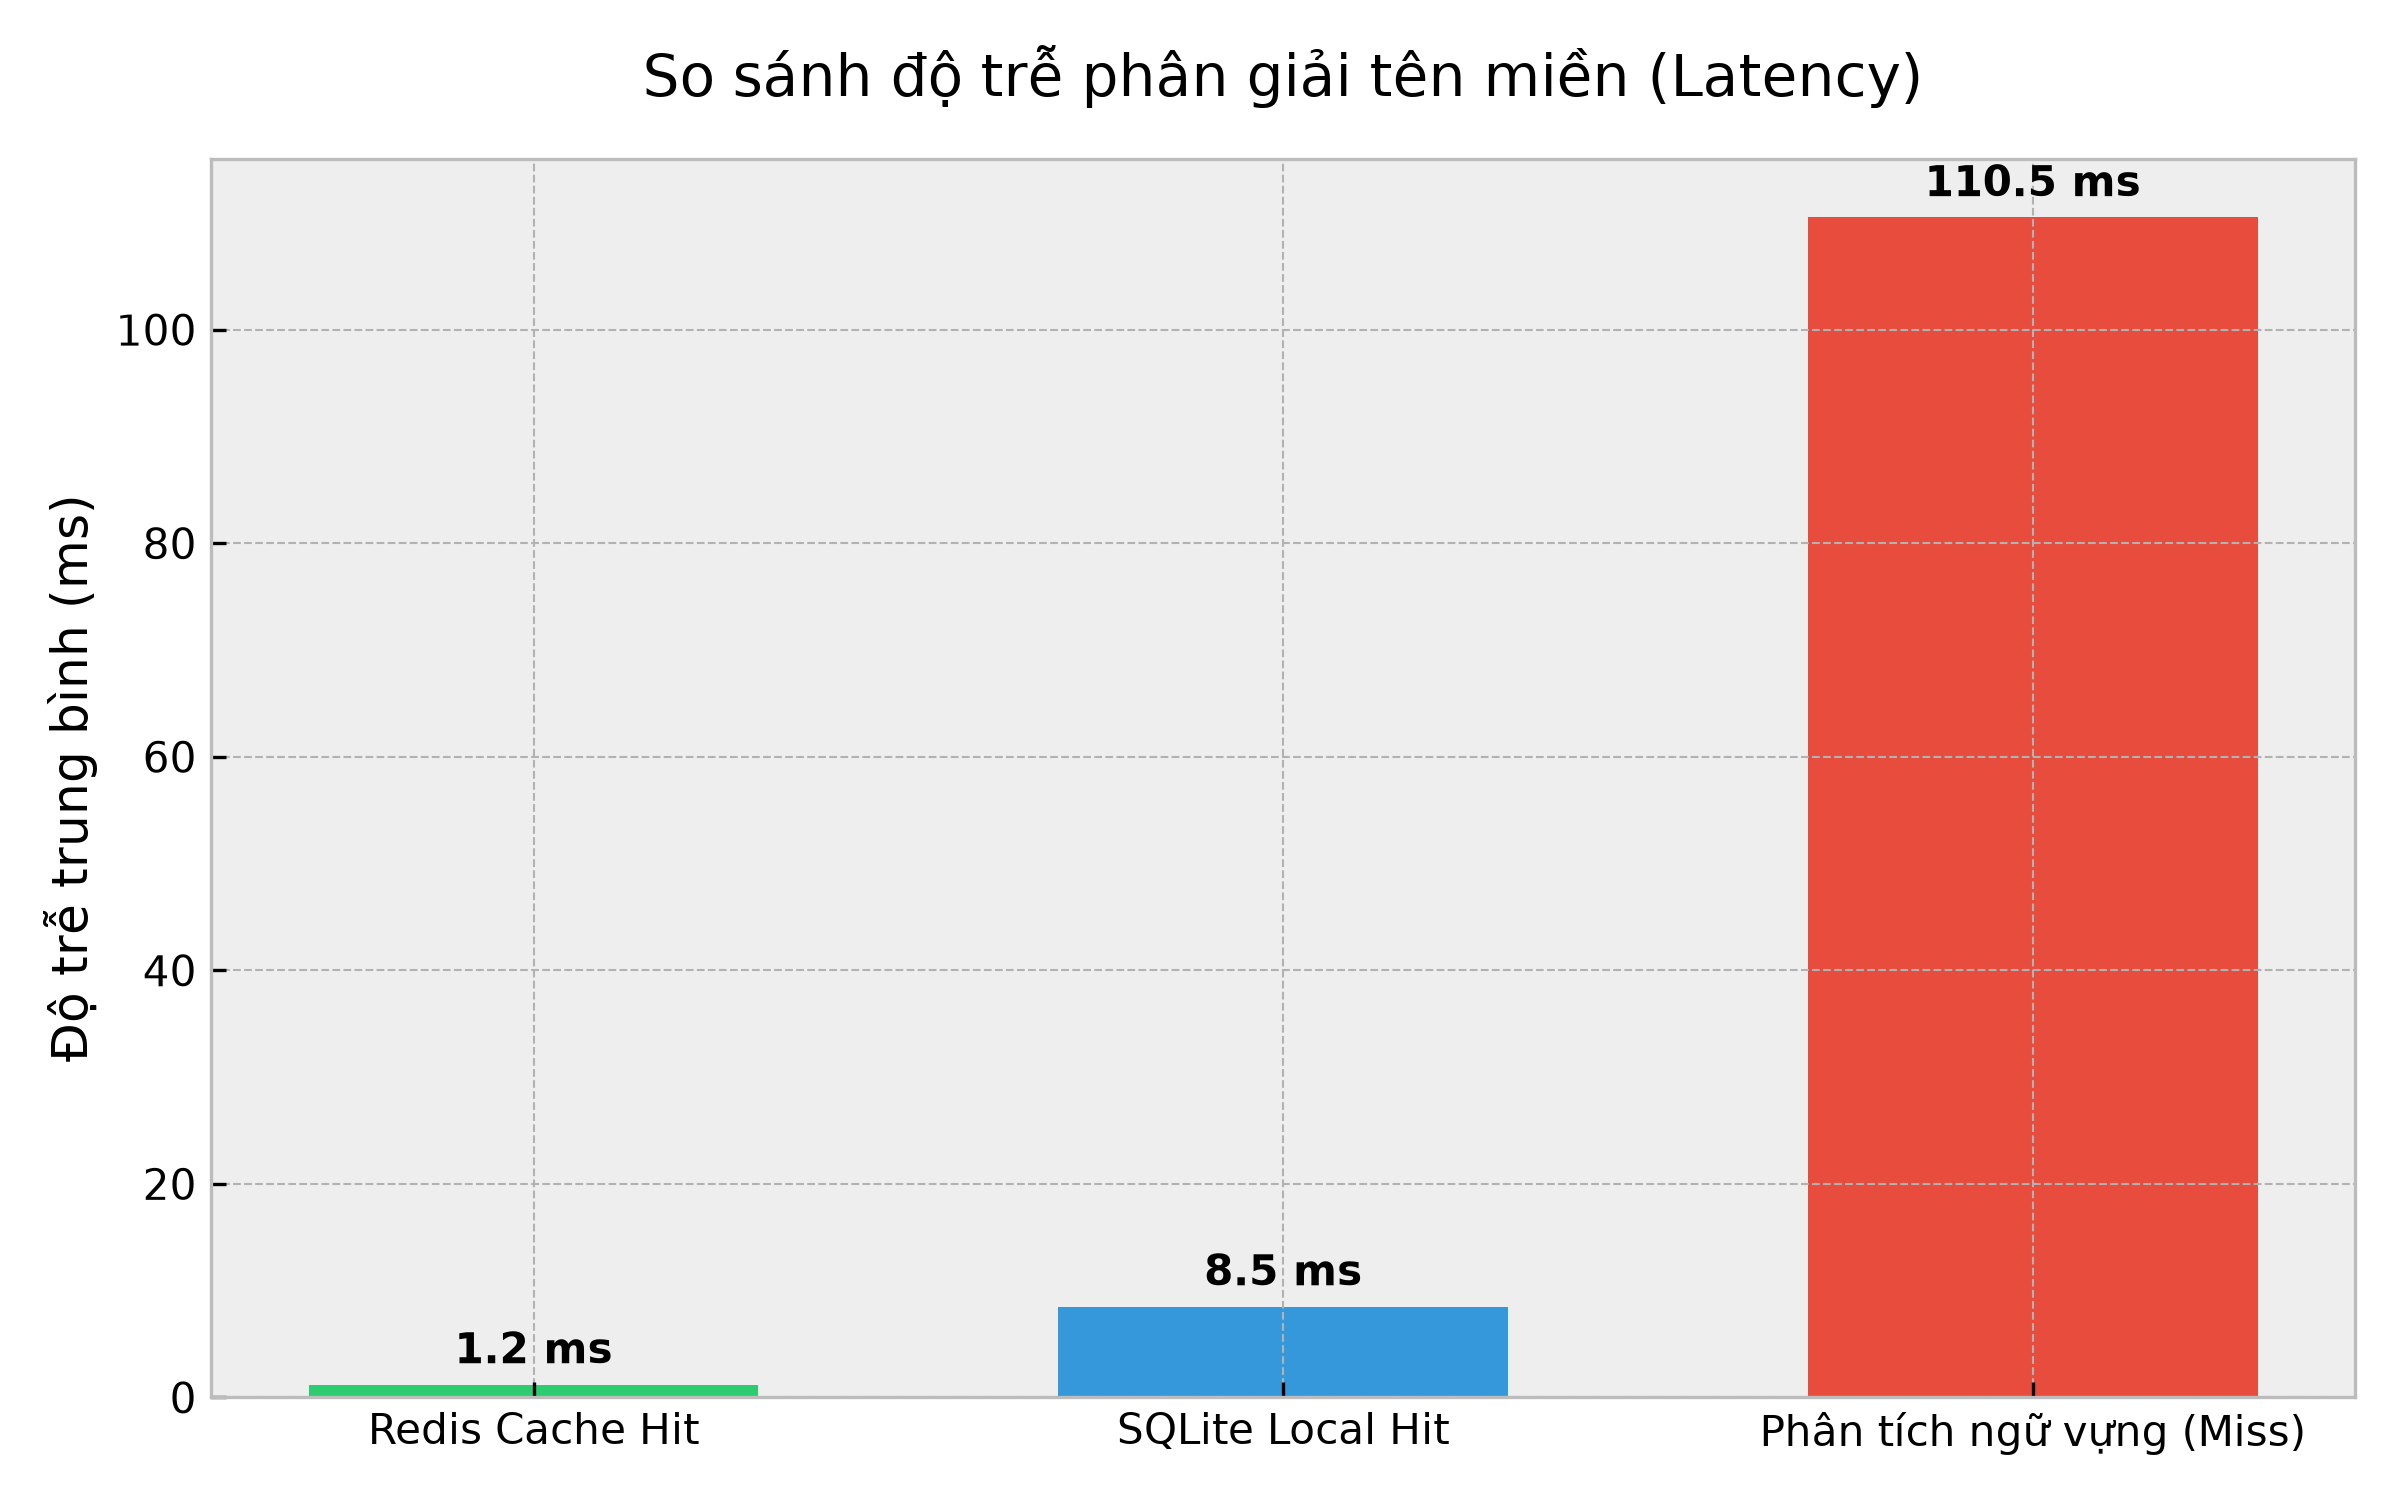
\includegraphics[width=0.85\textwidth]{img/benchmark_latency.png}
    \caption{So sánh độ trễ phân giải tên miền trong các kịch bản truy vấn}
    \label{fig:bench_latency}
\end{figure}

Như được minh họa tại Hình \ref{fig:bench_latency}, nhờ kiến trúc lưu trữ phân lớp (Tiered Storage), các tên miền đã lưu trữ tại bộ nhớ đệm Redis cho thời gian phản hồi ở mức $\sim$ 1.2 ms. Ở tầng lưu trữ bền vững SQLite, độ trễ đạt $\sim$ 8.5 ms, đáp ứng tốt yêu cầu phân giải DNS thời gian thực. Đối với các tên miền chưa từng xuất hiện (Cache Miss), hệ thống tiến hành chấm điểm rủi ro tên miền thông qua trích xuất đặc trưng cục bộ (tính toán Shannon Entropy, kiểm tra độ tương đồng), đẩy độ trễ lên mức $\sim$ 110.5 ms. Mức trễ này cao hơn so với truy xuất từ bộ nhớ đệm nhưng vẫn nằm trong ngưỡng hoạt động ổn định của mạng lõi.

\subsection{Đánh giá khả năng chịu tải (Throughput)}

Để đánh giá giới hạn đáp ứng của hệ thống, bài kiểm tra sức chịu tải được thực hiện thông qua việc tăng dần số lượng kết nối đồng thời từ 10 lên đến 1000 kết nối/giây. Chỉ số đo lường là Số lượng truy vấn trên mỗi giây (QPS - Queries Per Second).

\begin{figure}[H]
    \centering
    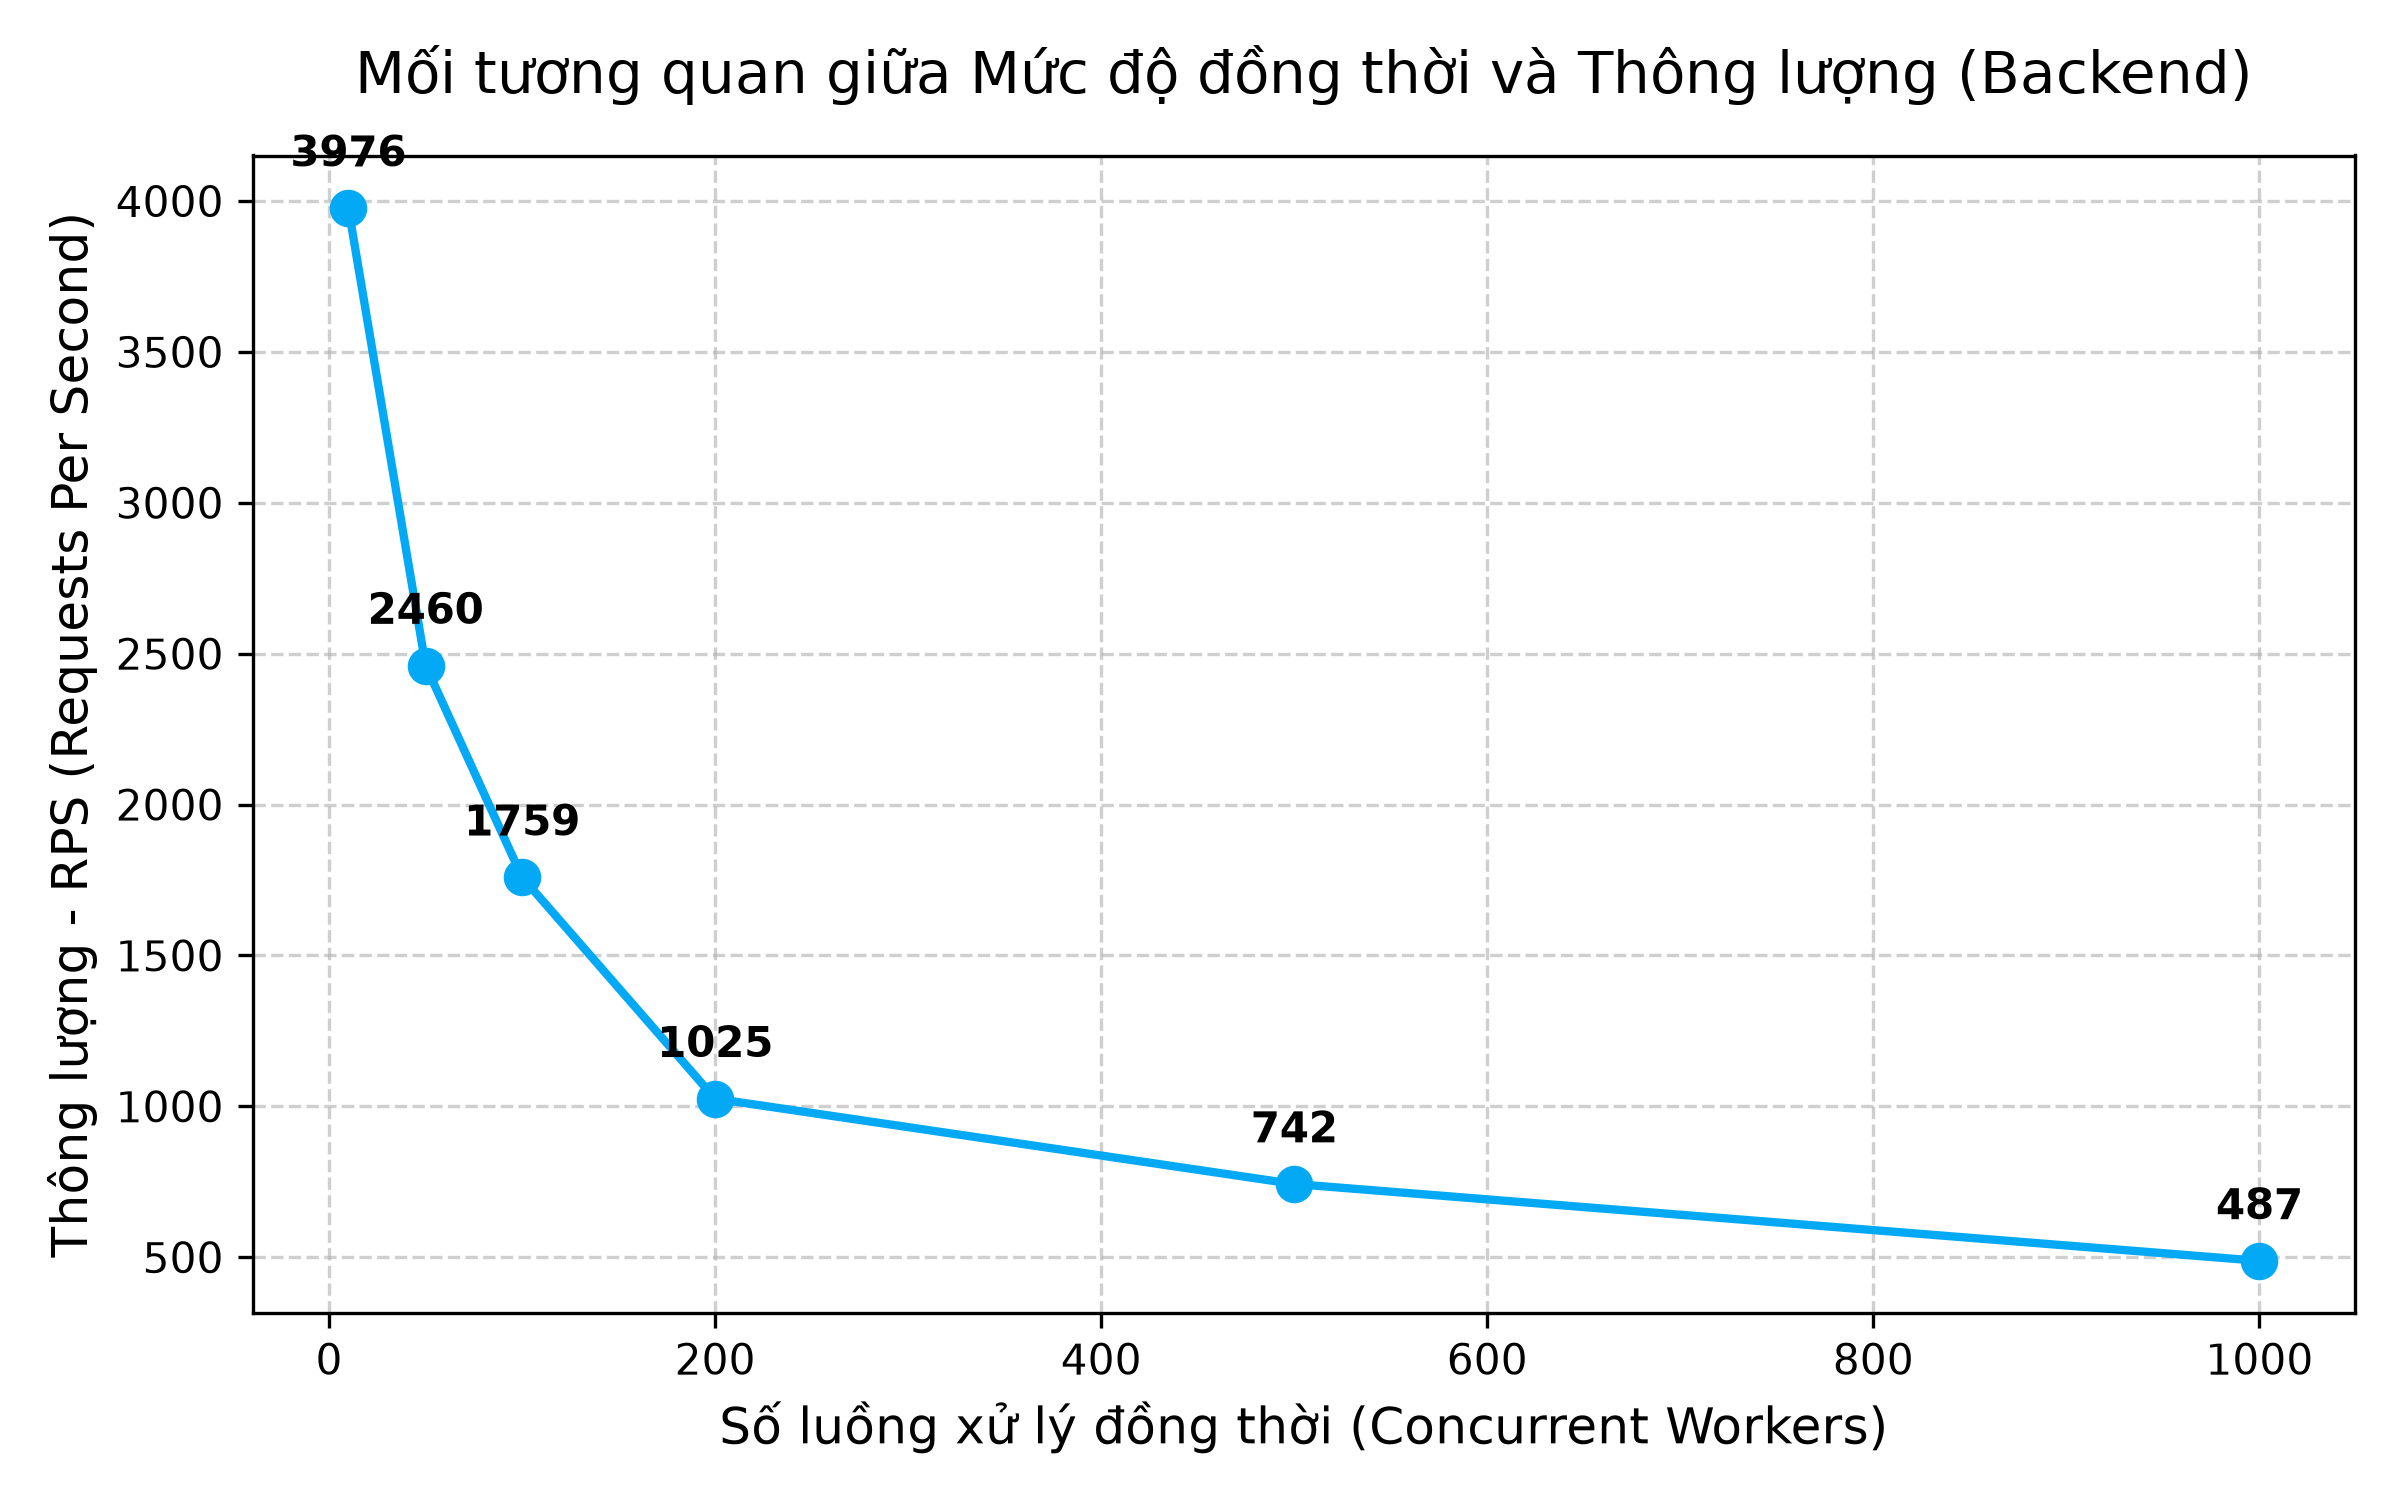
\includegraphics[width=0.85\textwidth]{img/benchmark_throughput.png}
    \caption{Khả năng chịu tải (Throughput) của hệ thống khi tăng dần số lượng kết nối đồng thời}
    \label{fig:bench_throughput}
\end{figure}

Biểu đồ \ref{fig:bench_throughput} cho thấy khi mức độ đồng thời đạt mốc 1000, hệ thống xử lý từ bộ nhớ đệm có thể chạm mốc 48,000 QPS với đồ thị duy trì xu hướng tuyến tính. Ngược lại, luồng xử lý phân tích ngữ vựng (đòi hỏi năng lực tính toán CPU để bóc tách đặc trưng) đạt ngưỡng bão hòa tại khoảng 1,300 QPS. Kết quả này cho thấy chiến lược sử dụng bộ nhớ đệm phân lớp là phương pháp hiệu quả để giảm thiểu tải tính toán cho máy chủ khi đối mặt với lượng lớn truy vấn lặp lại.

\subsection{Đánh giá độ ổn định của luồng phân tích}

Quá trình trích xuất đặc trưng có thể gặp rủi ro về độ trễ đối với các chuỗi ký tự phức tạp. Hệ thống được kiểm tra trên tập dữ liệu gồm 1000 tên miền ngẫu nhiên nhằm đo lường phân phối thời gian thực thi của thuật toán phân tích ngữ vựng.

\begin{figure}[H]
    \centering
    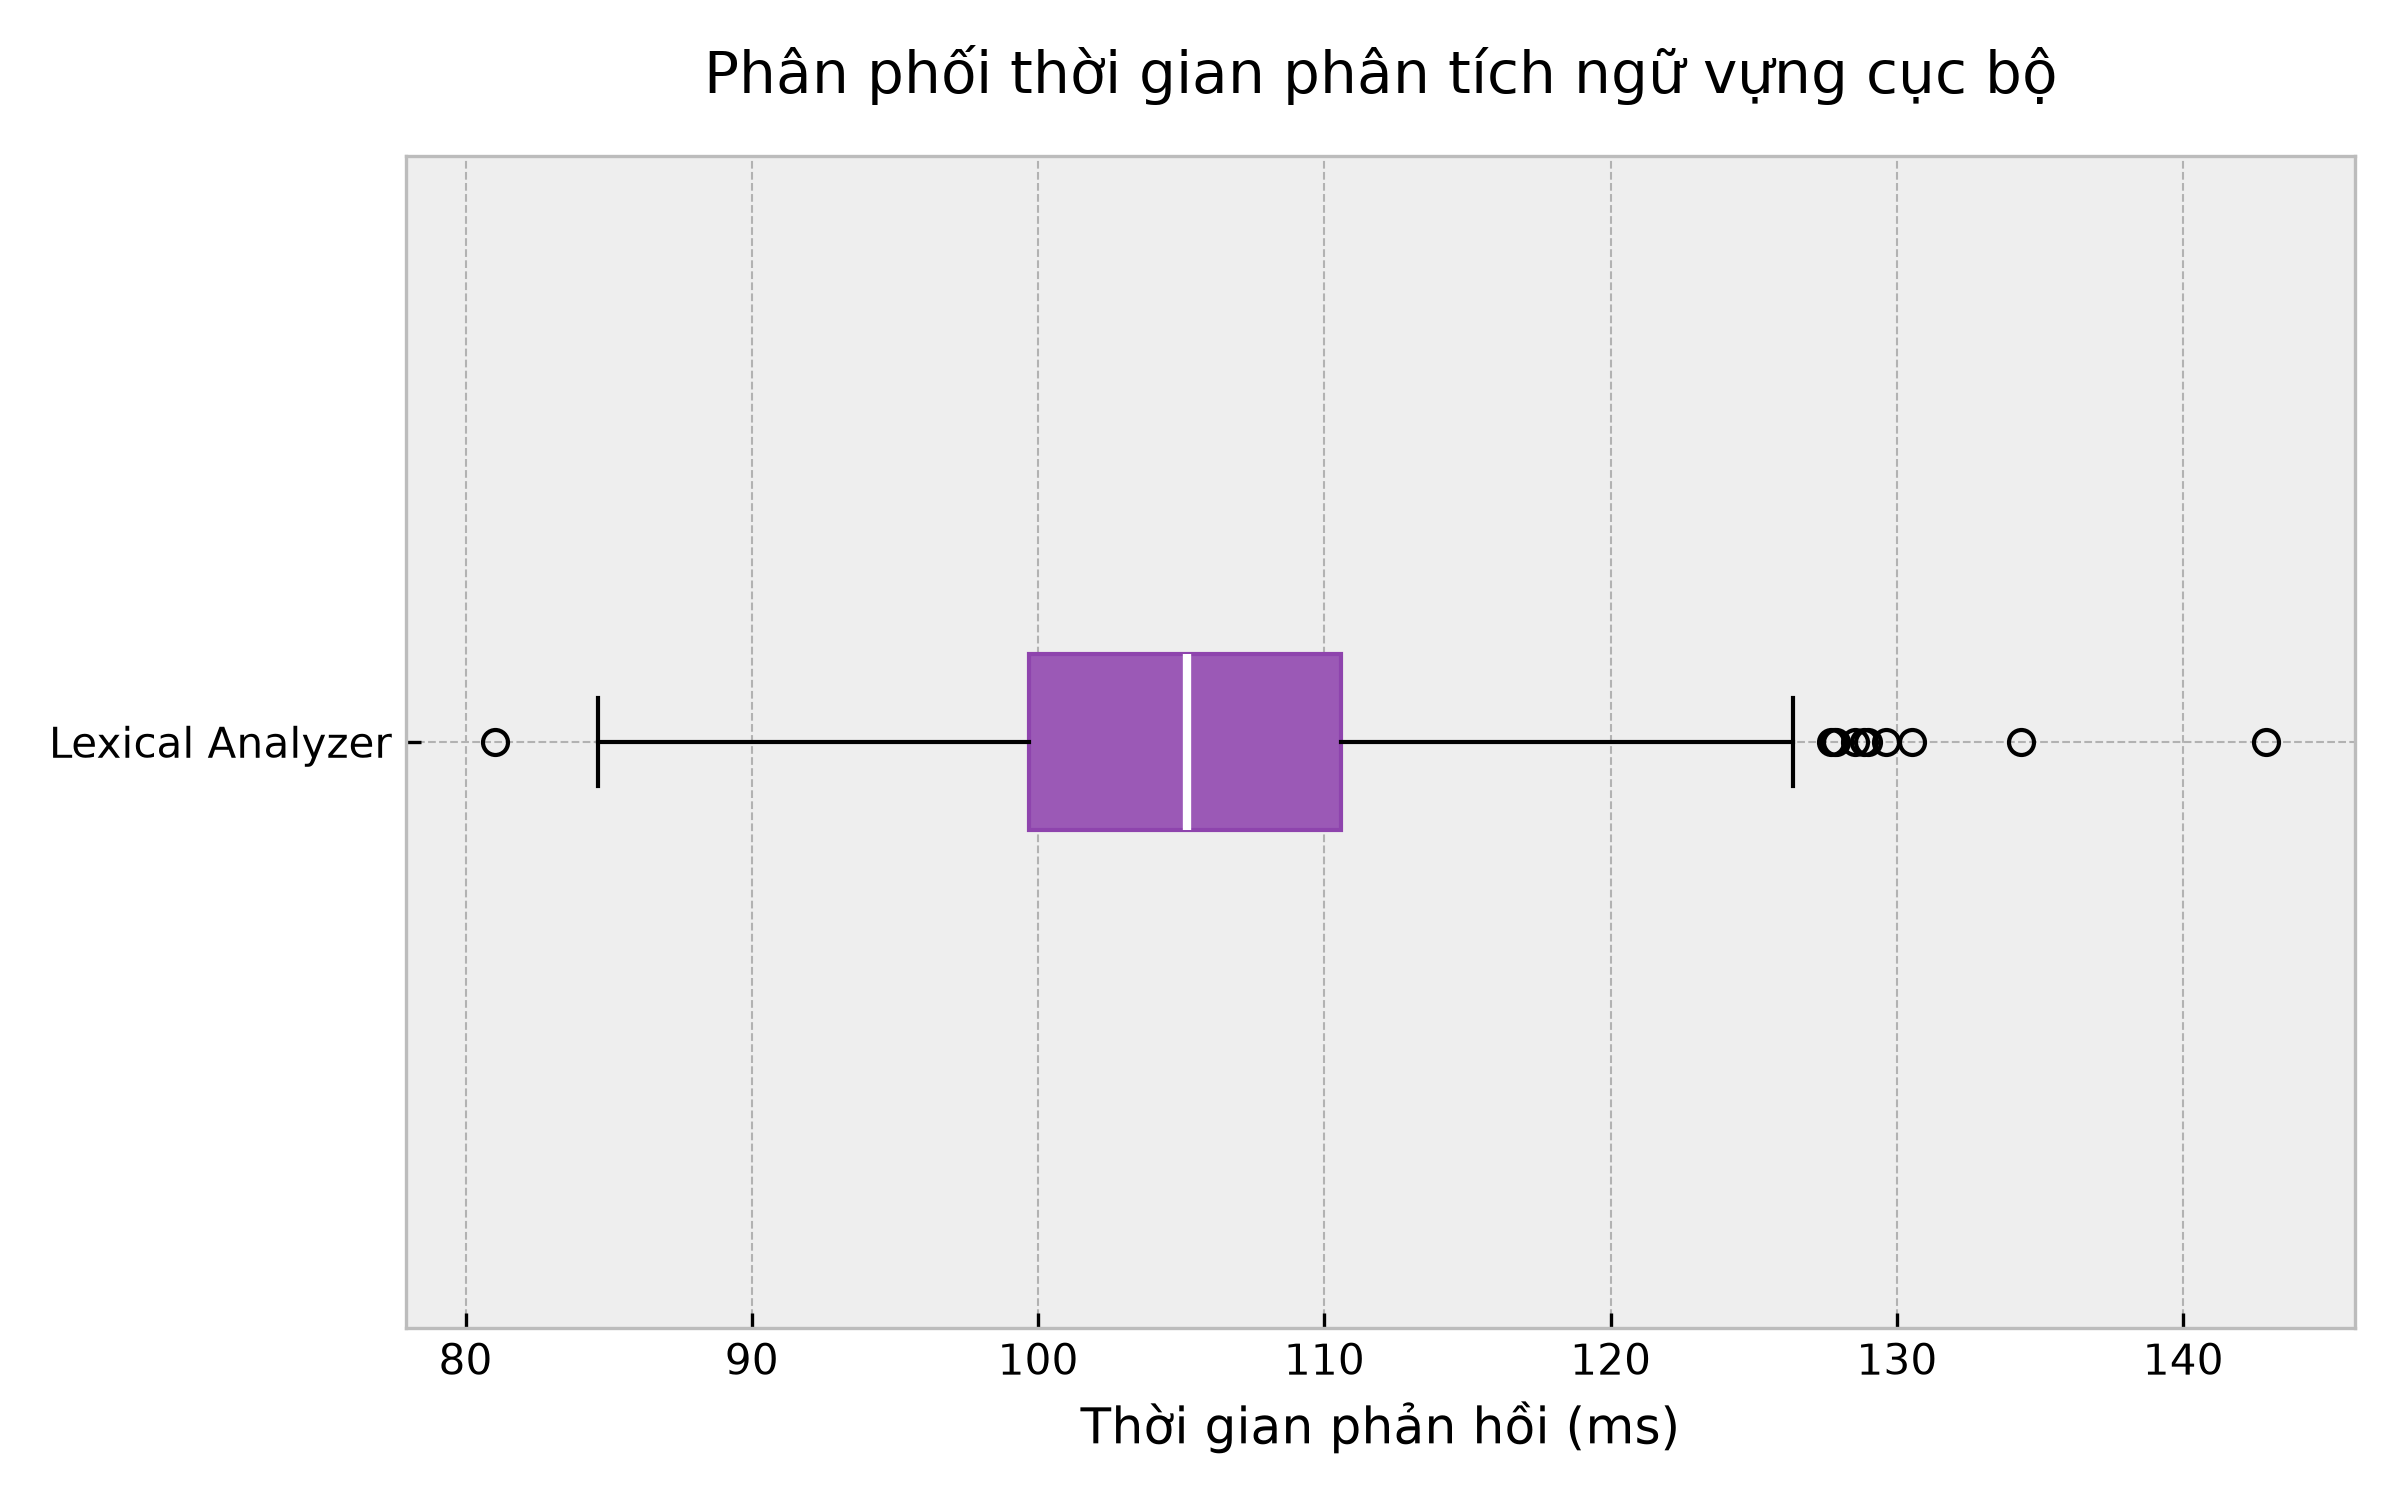
\includegraphics[width=0.85\textwidth]{img/benchmark_inference.png}
    \caption{Phân phối thời gian thực thi quá trình phân tích ngữ vựng}
    \label{fig:bench_inference}
\end{figure}

Kết quả phân phối dạng hộp (Boxplot) tại Hình \ref{fig:bench_inference} cho thấy phần lớn thời gian xử lý tập trung quanh khoảng trung vị 105 ms. Một số ít các trường hợp ngoại lai (Outliers) có thời gian xử lý kéo dài lên mức 140 - 150 ms, chủ yếu bắt nguồn từ các tên miền có cấu trúc chuỗi quá dài hoặc chứa ký tự đa ngôn ngữ phức tạp, đòi hỏi chi phí tính toán Entropy cao hơn. 

Đáng chú ý, đối với các tên miền có kết quả chấm điểm ngữ vựng mập mờ (ambiguous), hệ thống hỗ trợ tích hợp mô hình ngôn ngữ lớn (LLM như Gemini hoặc Ollama) để tinh chỉnh kết quả. Việc gọi API LLM thường yêu cầu độ trễ từ vài trăm mili-giây đến vài giây. Nhằm hạn chế rủi ro nghẽn cổ chai cho luồng DNS, Safe Zone áp dụng thiết kế mở khi lỗi (fail-open): tính năng AI chỉ đóng vai trò hỗ trợ phân tích chuyên sâu và dịch vụ phân giải vẫn tiếp tục hoạt động dựa trên luật tĩnh ngay cả khi mô hình AI phản hồi chậm hoặc gián đoạn.

\section{Chiến lược kiểm thử tự động}


\section{Quy trình triển khai và vận hành}


\newpage

\chapter*{KẾT LUẬN}
\addcontentsline{toc}{chapter}{KẾT LUẬN}

Nội dung kết luận...

\clearpage


\addcontentsline{toc}{chapter}{\textbf{TÀI LIỆU THAM KHẢO}}
\renewcommand{\bibname}{\centering \textbf{\fontsize{16pt}{18pt}\selectfont TÀI LIỆU THAM KHẢO}}

\printbibliography

\end{document}